\newpage
\section{Background on Algebraic Geometry and Combinatorics}\label{Appendix:A}

In this appendix, we provide essential background on convex geometry, polynomial support structures, and lattice path enumeration that facilitate understanding of the complexity analysis in Section~\ref{Section:Complexity}. For a detailed introduction to these topics, please refer to~\cite{cox2005using,sturmfels2002solving,bona2015handbook}.


\begin{definition}[Generic Property~\cite{cox2005using}]\label{def:generic}
	Fix degree bounds $d_1,\ldots,d_n$, and let $\mathcal{C}$ be the affine space over
	$\overline{\mathbb{K}}$ of the coefficient tuples of polynomial systems
	$(f_1,\ldots,f_n)$ with $\deg_{\xvec}(f_i)\le d_i$.
	A property $\mathcal{P}$ is said to hold \emph{generically} if there exists a
	Zariski open dense subset $U\subseteq \mathcal{C}$ such that $\mathcal{P}$ holds
	for every $(f_1,\ldots,f_n)\in U$.
\end{definition}


Equivalently, the property holds whenever a suitable nonzero polynomial in the input coefficients does not vanish; see~\cite[Chapter~3, \S5, Definition~(5.6), p.~115]{cox2005using}. The exceptional systems are contained in a proper algebraic subset. Over a finite base field, this definition is interpreted over its algebraic closure and does not by itself assert a probability of success for sampling in that finite field.


\begin{definition}[Convex Set and Convex Hull]
	A set $C \subset \mathbb{R}^n$ is \emph{convex} if for any two points $p, q \in C$, the line segment $\{(1-\lambda)p + \lambda q : \lambda \in [0,1]\}$ lies entirely in $C$. 
	
	For any set $S \subset \mathbb{R}^n$, its \emph{convex hull} $\text{conv}(S)$ is the smallest convex set containing $S$, equivalently:
	\[\text{conv}(S) = \left\{\sum_{i=1}^m \lambda_i s_i : s_i \in S, \lambda_i \geq 0, \sum_{i=1}^m \lambda_i = 1\right\}.\]
	Linear combinations of this form are called \emph{convex combinations}.
\end{definition}

\begin{definition}[Polytope]
	A \emph{polytope} is the convex hull of a finite set in $\mathbb{R}^n$. A \emph{lattice polytope} is a polytope whose vertices lie in $\mathbb{Z}^n$.
\end{definition}


\begin{definition}[Monomial Support]\label{def:support}
	For a polynomial $f = \sum_{\alpha} c_{\alpha} x^{\alpha}$ where $c_{\alpha} \in \mathbb{K}$ and $\alpha \in \mathbb{Z}_{\geq 0}^n$, the \emph{support} of $f$ is the set of exponent vectors corresponding to nonzero coefficients:
	\[\text{Supp}(f) = \{\alpha \in \mathbb{Z}_{\geq 0}^n : c_{\alpha} \neq 0\}.\]
\end{definition}

\begin{definition}[Newton Polytope]\label{def:newton}
	The \emph{Newton polytope} of a polynomial $f$ is the convex hull of its support:
	\[\text{NP}(f) = \text{conv}(\text{Supp}(f)) \subset \mathbb{R}^n.\]
	The Newton polytope records the "shape" or sparsity structure of $f$; the actual coefficient values do not affect $\text{NP}(f)$.
\end{definition}

\begin{definition}[Mixed and Unmixed Systems~\cite{DBLP:conf/stoc/KapurS96}]\label{def:mixed-unmixed}
	A polynomial system $\mathcal{F} = (f_1,\ldots,f_n)$ is called \emph{unmixed} if
	\[
	\mathrm{NP}(f_1)=\cdots=\mathrm{NP}(f_n).
	\]
	Otherwise, it is called \emph{mixed}.
\end{definition}


\begin{definition}[Minkowski Sum]\label{def:minkowski}
	For polytopes $P_1, P_2 \subset \mathbb{R}^n$, their {Minkowski sum} is:
	\[P_1 + P_2 = \{p_1 + p_2 : p_1 \in P_1, p_2 \in P_2\}.\]
	More generally, for $\lambda \geq 0$ and polytope $P$, define $\lambda P = \{\lambda p : p \in P\}$.
\end{definition}

\begin{proposition}[Properties of Minkowski Sum]
	\begin{enumerate}
		\item The Minkowski sum of polytopes is a polytope.
		\item The Minkowski sum of lattice polytopes is a lattice polytope.
		\item For polytopes $P, Q$ and $\lambda, \mu \geq 0$: $\lambda(P + Q) = \lambda P + \lambda Q$ and $(\lambda + \mu)P = \lambda P + \mu P$.
	\end{enumerate}
\end{proposition}

\begin{proposition}[Newton Polytope of Products {\cite[Fact~3.2]{DBLP:conf/stoc/KapurS96}}]\label{prop:newton-product}
	For nonzero polynomials $f, g \in \mathbb{K}[x_1, \ldots, x_n]$:
	\[\text{NP}(fg) = \text{NP}(f) + \text{NP}(g).\]
\end{proposition}

\begin{proposition}[Faces of Minkowski Sums]\label{prop:minkowski-faces}
	Let $P_1, \ldots, P_r \subset \mathbb{R}^n$ be polytopes, and let $P = P_1 + \cdots + P_r$ be their Minkowski sum. Then every face $P'$ of $P$ can be expressed as a Minkowski sum:
	\[P' = P'_1 + \cdots + P'_r,\]
	where each $P'_i$ is a face of $P_i$.
\end{proposition}

\begin{definition}[Lattice Path]\label{def:lattice_path}
	A \emph{lattice path} in $\mathbb{Z}_{\geq 0}^2$ from $(0,0)$ to $(u,w)$ is a sequence of points
	\[
	(x_0,y_0),(x_1,y_1),\ldots,(x_k,y_k)
	\]
	such that $(x_0,y_0)=(0,0)$, $(x_k,y_k)=(u,w)$, and for each $i=0,1,\ldots,k-1$ we have either
	\[
	(x_{i+1},y_{i+1})=(x_i+1,y_i)\quad\text{(a right step)}
	\]
	or
	\[
	(x_{i+1},y_{i+1})=(x_i,y_i+1)\quad\text{(an up step)}.
	\]
	All points of the path lie in $\mathbb{Z}_{\geq 0}^2$. Such a path consists of exactly $u$ horizontal steps and $w$ upward steps; the \emph{height} of a horizontal step is the $y$-coordinate at which it is taken.
	The {number of lattice paths} refers to the total number of distinct lattice paths satisfying these conditions.
\end{definition}

\newpage

\section{Proof of Lemma~\ref{lem:fc_polytope}}
\label{appendix:proof_lemma_fc}

\begin{proof}
	We establish the equality by showing both inclusions.
	
	\paragraph{Setup.}
	For each $k \in \{1, \ldots, n\}$, define
	\begin{equation*}
		P_k := \{(i_1, \ldots, i_k, 0, \ldots, 0) \in \mathbb{Z}_{\geq 0}^n : i_1 + \cdots + i_k \leq d_k\}.
	\end{equation*}
	By definition of the Iterated-Simplex Polynomial, whose coefficients over $\mathbb{Z}$ are positive,
	\begin{equation*}
		\operatorname{Supp}(I_{d_1, d_2, \ldots, d_n}) = P_1 + P_2 + \cdots + P_n,
	\end{equation*}
	where $+$ denotes the Minkowski sum. Define the target set:
	\begin{equation*}
		Q_n := \left\{(\alpha_1, \ldots, \alpha_n) \in \mathbb{Z}_{\geq 0}^n : \sum_{\ell=n-j+1}^{n} \alpha_\ell \leq \sum_{i=1}^{j} d_{n-i+1} \text{ for all } j \in \{1, \ldots, n\}\right\}.
	\end{equation*}
	
	\paragraph{Inclusion $P_1 + \cdots + P_n \subseteq Q_n$.}
	Let $(\alpha_1, \ldots, \alpha_n) \in P_1 + \cdots + P_n$. Then there exist $(i_1^{(k)}, \ldots, i_n^{(k)}) \in P_k$ for $k = 1, \ldots, n$ such that
	\begin{equation*}
		(\alpha_1, \ldots, \alpha_n) = \sum_{k=1}^{n} (i_1^{(k)}, \ldots, i_n^{(k)}).
	\end{equation*}
	
	Fix $j \in \{1, \ldots, n\}$ and consider the last $j$ components. For each $k \in \{n-j+1, \ldots, n\}$, by the definition of $P_k$, we have
	\begin{equation*}
		\sum_{\ell=n-j+1}^{n} i_\ell^{(k)} \leq d_k.
	\end{equation*}
	
	Therefore,
	\begin{align*}
		\sum_{\ell=n-j+1}^{n} \alpha_\ell 
		&= \sum_{\ell=n-j+1}^{n} \sum_{k=1}^{n} i_\ell^{(k)} 
		= \sum_{k=n-j+1}^{n} \sum_{\ell=n-j+1}^{n} i_\ell^{(k)} \\[0.3em]\notag
		&\leq \sum_{k=n-j+1}^{n} d_k 
		= \sum_{i=1}^{j} d_{n-i+1}.
	\end{align*}
	
	This shows $(\alpha_1, \ldots, \alpha_n) \in Q_n$.
	
	\paragraph{Inclusion $Q_n \subseteq P_1 + \cdots + P_n$.}
	The strategy is to construct the decomposition by greedily moving mass from the last coordinates of $\alpha$ into $P_n$ (which can absorb up to $d_n$ units of total mass), while keeping the prefix $(\alpha_1',\ldots,\alpha_{n-1}',0)$ inside $Q_{n-1}$. We proceed by induction on $n$. For $n = 1$, clearly $P_1 = Q_1$.
	
	Assume $n \geq 2$ and $P_1 + \cdots + P_{n-1} = Q_{n-1}$, where $Q_{n-1}$ is the set attached to the truncated sequence $(d_1,\ldots,d_{n-1})$, viewed as a subset of $\mathbb{Z}_{\geq 0}^{n-1} \times \{0\}$.
	Let $(\alpha_1, \ldots, \alpha_n) \in Q_n$. We construct a decomposition
	\begin{equation*}
		(\alpha_1, \ldots, \alpha_n) = (\alpha_1', \ldots, \alpha_{n-1}', 0) + (\alpha_1'', \ldots, \alpha_n'')
	\end{equation*}
	with $(\alpha_1', \ldots, \alpha_{n-1}', 0) \in Q_{n-1}$ and $(\alpha_1'', \ldots, \alpha_n'') \in P_n$.
	
	We define the decomposition recursively for $j = 1, \ldots, n$. At step $j$, if
	\begin{equation*}
		\alpha_{n-j+1} + \sum_{\ell=n-j+2}^{n-1} \alpha_\ell' \leq \sum_{i=2}^{j} d_{n-i+1}
	\end{equation*}
	(with the convention that the sums $\sum_{\ell=n-j+2}^{n-1}\alpha_\ell'$ and $\sum_{i=2}^{j}d_{n-i+1}$ are empty---and therefore equal to $0$---when $j=1$), set
	\(\alpha_{n-j+1}' := \alpha_{n-j+1}\), 
    \(\alpha_{n-j+1}'' := 0\).
	Otherwise, set
	\begin{equation*}
		\alpha_{n-j+1}' := \sum_{i=2}^{j} d_{n-i+1} - \sum_{\ell=n-j+2}^{n-1} \alpha_\ell', \quad 
		\alpha_{n-j+1}'' := \alpha_{n-j+1} - \alpha_{n-j+1}'.
	\end{equation*}
	Here $\sum_{i=2}^{j} d_{n-i+1}=\sum_{k=n-j+1}^{n-1} d_k$ is precisely the budget that $Q_{n-1}$ allows for the suffix starting at index $n-j+1$; note also that this budget increases by $d_{n-j+1}\ge 0$ from step $j-1$ to step $j$, so $\alpha_{n-j+1}'\ge 0$ in the second case. At $j=1$ the budget is the empty sum $0$, so the step forces $\alpha_n'=0$.
	
	In both cases,
	\begin{equation*}
		\sum_{\ell=n-j+1}^{n-1} \alpha_\ell' \leq \sum_{i=2}^{j} d_{n-i+1},
	\end{equation*}
	which establishes $(\alpha_1', \ldots, \alpha_{n-1}', 0) \in Q_{n-1}$.
	
	To verify $(\alpha_1'', \ldots, \alpha_n'') \in P_n$, we need $\sum_{\ell=1}^{n} \alpha_\ell'' \leq d_n$. If the second case never occurs, then $\alpha''=0$ and there is nothing to prove. Otherwise, let $j$ be the \emph{largest} index at which the second case occurs; then $\alpha_\ell''=0$ for every $\ell<n-j+1$, and since the second case saturates the budget at step $j$ we obtain
	\begin{align*}
		\sum_{\ell=1}^{n} \alpha_\ell''=\sum_{\ell=n-j+1}^{n} \alpha_\ell''
		&= \alpha_{n-j+1} -\!\left(\sum_{i=2}^{j} d_{n-i+1} - \sum_{\ell=n-j+2}^{n-1} \alpha_\ell'\right)\!+\!\sum_{\ell=n-j+2}^{n} \alpha_\ell'' \\[0.3em]
		&= \sum_{\ell=n-j+1}^{n} \alpha_\ell\!-\!\sum_{i=2}^{j} d_{n-i+1}
		\leq \sum_{i=1}^{j} d_{n-i+1}\!-\!\sum_{i=2}^{j} d_{n-i+1}
		= d_n,
	\end{align*}
	where the inequality follows from the definition of $Q_n$.
	
	By the induction hypothesis,
	\begin{equation*}
		(\alpha_1, \ldots, \alpha_n) \in Q_{n-1} + P_n \subseteq P_1 + \cdots + P_n.
	\end{equation*}
	
Combining the two inclusions gives $\operatorname{Supp}(I_{d_1,\ldots,d_n})=P_1+\cdots+P_n=Q_n$.
    \qed
\end{proof}


\newpage
\section{Experimental Validation for Dixon Matrix Size Bound}\label{appendix:experimental_bound}

We provide numerical comparisons between our Fuss--Catalan bound (FC Bound, Corollary~\ref{cor:three_bounds}(2)), Unrestricted bound (Corollary~\ref{cor:three_bounds}(1)), the volume comparison bound~\eqref{eq:Dixon_volume_bound}, motivated by~\cite[Theorem~4.3]{DBLP:conf/stoc/KapurS96} and verified in Section~\ref{Subsection:Matrix_Size}, and the trivial variable-based bound~\eqref{eq:Dixon_var_bound}. Table~\ref{tab:dixon_matrix_comparison} shows the bounds alongside the actual Dixon matrix sizes computed from randomly generated dense $(n;d)$-systems over $\mathbb{F}_p$ with $p=2^{31}-159$; generic attainment is subject to the characteristic hypothesis in Lemma~\ref{lem:dixon_fc_bound}, and we record the field used for reproducibility. The ``True Size'' column reports the actual row/column dimension of the Dixon matrix observed in our experiments. For each pair $(n,d)$ we sampled $20$ independent, fully dense systems of $n$ equations, all of total degree $d$, with all coefficients drawn uniformly and independently from $\Fp$; the observed size agreed across all samples. It is the support dimension $D(\mathcal{F})$, not $\operatorname{rank}\mathcal{M}$ (Remark~\ref{rem:support_vs_rank}).

\begin{table}[htbp]
	\centering
	\caption{Comparison of Dixon Matrix Size Bounds}
	\label{tab:dixon_matrix_comparison}
	\begin{tabular}{ccccccc}
		\toprule
		$n$ & $d$ & FC Bound & Unrestricted Bound & Volume Bound & Variable Bound & True Size \\
		\midrule
		3 & 2 & 5 & 6 & 6 & 8 & 5 \\
		3 & 3 & 12 & 15 & 13 & 18 & 12 \\
		3 & 4 & 22 & 28 & 24 & 32 & 22 \\
		3 & 5 & 35 & 45 & 37 & 50 & 35 \\
		
		4 & 2 & 14 & 20 & 21 & 48 & 14 \\
		4 & 3 & 55 & 84 & 72 & 162 & 55 \\
		4 & 4 & 140 & 220 & 170 & 384 & 140 \\
		4 & 5 & 285 & 455 & 333 & 750 & 285 \\
		
		5 & 2 & 42 & 70 & 83 & 384 & 42 \\
		5 & 3 & 273 & 495 & 421 & 1944 & 273 \\
		5 & 4 & 969 & 1820 & 1333 & 6144 & 969 \\
		5 & 5 & 2530 & 4845 & 3255 & 15000 & 2530 \\
		
		6 & 2 & 132 & 252 & 345 & 3840 & 132 \\
		6 & 3 & 1428 & 3003 & 2624 & 29160 & 1428 \\
		6 & 4 & 7084 & 15504 & 11059 & 122880 & 7084 \\
		6 & 5 & 23751 & 53130 & 33750 & 375000 & 23751 \\
		
		7 & 2 & 429 & 924 & 1493 & 46080 & 429 \\
		7 & 3 & 7752 & 18564 & 17017 & 524880 & 7752 \\
		
		8 & 2 & 1430 & 3432 & 6657 & 645120 & 1430 \\
		
		9 & 2 & 4862 & 12870 & 30368 & 10321920 & 4862 \\
		
		10 & 2 & 16796 & 48620 & 141093 & 185794560 & 16796 \\
		
		\bottomrule
	\end{tabular}
\end{table}

\newpage

\section{Detailed Derivation of Complexity Ratios in Table~\ref{tab:complexity_formulas}}
\label{Appendix:Derivation}

This appendix gives the step-by-step derivation of the ``Ratio to Dixon'' column in Table~\ref{tab:complexity_formulas}. The three Gr\"obner-basis ratios have the same orders whether $n\ge2$ is fixed and $d\to\infty$, or $d\ge2$ is fixed and $n\to\infty$. The change-of-order ratios depend on the direction of growth, so we give both estimates for FGLM below. In the ratios, $\widehat{\mathcal T}_M$ denotes the expression inside the displayed cost bound for method $M$, with logarithmic factors omitted.

For a well-determined $(n;d)$-system, we use the Dixon resultant complexity as the baseline:
\[
\mathcal T_{\mathrm{Dixon}}
=\widetilde{\mathcal O}\!\left(nd\left(\frac{1}{n(d-1)+1}\binom{nd}{n}\right)^\omega\right).
\]

\paragraph{Gr\"obner Basis Classical~\cite{Faugere2004}}

The complexity is
\[
\mathcal T_{\mathrm{GB}}
=\mathcal O\!\left(\binom{n+d_{\mathrm{reg}}}{d_{\mathrm{reg}}}^\omega\right).
\]
With $d_{\mathrm{reg}}=n(d-1)+1$, this becomes
\[
\mathcal T_{\mathrm{GB}}
=\mathcal O\!\left(\binom{nd+1}{n}^\omega\right).
\]
Using the binomial identity
\[
\binom{nd+1}{n}=\frac{nd+1}{nd-n+1}\binom{nd}{n},
\]
we compute the ratio:
\begin{align*}
\frac{\widehat{\mathcal T}_{\mathrm{GB}}}{\widehat{\mathcal T}_{\mathrm{Dixon}}}
&=\frac{\binom{nd+1}{n}^{\omega}}{nd\left(\frac{1}{n(d-1)+1}\binom{nd}{n}\right)^\omega}\\
&=\frac{(nd+1)^\omega}{nd}
=(nd)^{\omega-1}\left(1+\frac{1}{nd}\right)^\omega\\
&\sim(nd)^{\omega-1}.
\end{align*}

\paragraph{Gr\"obner Basis F5 Bound~\cite{DBLP:journals/jsc/BardetFS15,DBLP:journals/tosc/BariantBLP22}}

The complexity is
\[
\mathcal T_{\mathrm{F5}}
=\mathcal O\!\left(n\,d_{\mathrm{reg}}\binom{n+d_{\mathrm{reg}}-1}{d_{\mathrm{reg}}}^{\omega}\right).
\]
Substituting $d_{\mathrm{reg}}=n(d-1)+1$ gives
\[
\mathcal T_{\mathrm{F5}}
=\mathcal O\!\left(n\bigl(n(d-1)+1\bigr)\binom{nd}{n-1}^{\omega}\right).
\]
Using
\[
\binom{nd}{n-1}=\frac{n}{nd-n+1}\binom{nd}{n},
\]
the ratio becomes
\begin{align*}
\frac{\widehat{\mathcal T}_{\mathrm{F5}}}{\widehat{\mathcal T}_{\mathrm{Dixon}}}
&=\frac{n\bigl(n(d-1)+1\bigr)\binom{nd}{n-1}^{\omega}}{nd\left(\frac{1}{n(d-1)+1}\binom{nd}{n}\right)^\omega}\\
&=\frac{n^{\omega+1}(nd-n+1)}{nd}\\
&=n^{\omega+1}\left(1-\frac1d+\frac1{nd}\right)
\sim n^{\omega+1}.
\end{align*}

\paragraph{Gr\"obner Basis rectangular~\cite{DBLP:journals/jsc/BardetFS15}}

The bound comes from the Macaulay matrix at degree $d_{\mathrm{reg}}$. It has $r=n\binom{n+d_{\mathrm{reg}}-d}{n}$ rows and $c=\binom{n+d_{\mathrm{reg}}}{n}$ columns. Its row echelon form can be computed in $O(rc\varrho^{\omega-2})$ operations, where $\varrho\le c$ is the rank~\cite{storjohann2000algorithms}. Thus
\[
\mathcal T_{\mathrm{rect}}
=\mathcal O\!\left(n\binom{n+d_{\mathrm{reg}}-d}{n}
\binom{n+d_{\mathrm{reg}}}{n}^{\omega-1}\right).
\]
After substituting $d_{\mathrm{reg}}=n(d-1)+1$, this becomes
\[
\mathcal T_{\mathrm{rect}}
=\mathcal O\!\left(n\binom{(n-1)d+1}{n}\binom{nd+1}{n}^{\omega-1}\right).
\]
Applying the same binomial identity as above gives
\begin{align*}
\frac{\widehat{\mathcal T}_{\mathrm{rect}}}{\widehat{\mathcal T}_{\mathrm{Dixon}}}
&=\frac{n\binom{nd-d+1}{n}\binom{nd+1}{n}^{\omega-1}}{nd\left(\frac{1}{n(d-1)+1}\binom{nd}{n}\right)^\omega}\\
&=\frac{\binom{nd-d+1}{n}}{\binom{nd}{n}}
\frac{nd-n+1}{d}(nd+1)^{\omega-1}.
\end{align*}
For $n$ fixed and $d\to\infty$,
\[
\frac{\binom{nd-d+1}{n}}{\binom{nd}{n}}
=\prod_{i=0}^{n-1}\frac{nd-d+1-i}{nd-i}
\longrightarrow\left(1-\frac1n\right)^n.
\]
Consequently,
\[
\frac{\widehat{\mathcal T}_{\mathrm{rect}}}{\widehat{\mathcal T}_{\mathrm{Dixon}}}
\sim\left(1-\frac1n\right)^n n^\omega d^{\omega-1}
=\Theta\!\left(n^\omega d^{\omega-1}\right),
\]
where $1/4\le(1-1/n)^n<e^{-1}$ for $n\ge2$. More generally, the binomial quotient above is between $(1-1/n)^n$ and $1$ for all $n,d\ge2$. Combining this uniform bound with the exact expressions for the classical and F5 ratios gives
\[
\frac{\widehat{\mathcal T}_{\mathrm{GB}}}{\widehat{\mathcal T}_{\mathrm{Dixon}}}
=\Theta\!\left((nd)^{\omega-1}\right),\qquad
\frac{\widehat{\mathcal T}_{\mathrm{F5}}}{\widehat{\mathcal T}_{\mathrm{Dixon}}}
=\Theta\!\left(n^{\omega+1}\right),\qquad
\frac{\widehat{\mathcal T}_{\mathrm{rect}}}{\widehat{\mathcal T}_{\mathrm{Dixon}}}
=\Theta\!\left(n^\omega d^{\omega-1}\right).
\]
Thus the three Gr\"obner-basis rows retain exactly the orders displayed in Table~\ref{tab:complexity_formulas} in either standard direction of growth. Their leading constants may differ between the two directions; the statement is an order comparison, not a uniform joint asymptotic equivalence.

\paragraph{FGLM~\cite{DBLP:journals/jsc/FaugereGLM93,DBLP:journals/tosc/KoschatkoLR24}}

The complexity estimate, excluding construction of the multiplication matrices, is
\[
\mathcal T_{\mathrm{FGLM}}
=\mathcal O(n\,d_{\mathcal I}^{\omega})
=\mathcal O(n\,d^{n\omega}).
\]
For $n$ fixed and $d\to\infty$, the Fuss--Catalan formula gives
\begin{equation}\label{eq:fc_high_degree}
C_n^{(d)}
=\frac1{n!}\prod_{j=0}^{n-2}(nd-j)
=\frac{n^{n-1}}{n!}d^{n-1}\bigl(1+O_n(d^{-1})\bigr).
\end{equation}
Substituting this expansion into the ratio yields
\begin{align*}
\frac{\widehat{\mathcal T}_{\mathrm{FGLM}}}{\widehat{\mathcal T}_{\mathrm{Dixon}}}
&=\frac{n\,d^{n\omega}}{nd\left(C_n^{(d)}\right)^\omega}\\
&\sim\frac{n\,d^{n\omega}}{nd\left(\frac{n^{n-1}}{n!}\right)^\omega d^{(n-1)\omega}}\\
&=\left(\frac{n!}{n^{n-1}}\right)^\omega d^{\omega-1}.
\end{align*}
Stirling bounds simplify the factorial coefficient to
\begin{equation}\label{eq:factorial_coefficient}
\left(\frac{n!}{n^{n-1}}\right)^\omega
=\Theta\!\left(n^{3\omega/2}e^{-n\omega}\right),
\end{equation}
with constants depending only on $\omega$. Hence the ratio in the table is
\[
\frac{\widehat{\mathcal T}_{\mathrm{FGLM}}}{\widehat{\mathcal T}_{\mathrm{Dixon}}}
=\Theta\!\left(n^{3\omega/2}d^{\omega-1}e^{-n\omega}\right).
\]
The factorial expression is the exact leading coefficient for fixed $n$; the $e^{-n\omega}$ form displays its order of magnitude as a function of $n$. The high-degree expansion~\eqref{eq:fc_high_degree} is not a uniform joint limit in $(n,d)$.

\paragraph{BNS Change of Order~\cite{BerthomieuNeigerSafey2022}}

Under the shape and stability assumptions of~\cite[Theorem~1.1]{BerthomieuNeigerSafey2022}, the complexity is
\[
\mathcal T_{\mathrm{BNS}}
=\widetilde{\mathcal O}\!\left(t^{\omega-1}d_{\mathcal I}\right).
\]
Here $t$ counts the grevlex basis elements whose leading monomial is divisible by the smallest variable. For the generic-system estimate, use $d_{\mathcal I}=d^n$ and $t=\Theta(d^{n-1}/\sqrt n)$ as in~\cite[Section~6.2 and Table~1]{BerthomieuNeigerSafey2022}. Substitution gives
\begin{align*}
\mathcal T_{\mathrm{BNS}}
&=\widetilde{\mathcal O}\!\left(
\bigl(d^{n-1}n^{-1/2}\bigr)^{\omega-1}d^n\right)\\
&=\widetilde{\mathcal O}\!\left(n^{-(\omega-1)/2}d^{n\omega-\omega+1}\right).
\end{align*}
Using~\eqref{eq:fc_high_degree} and then~\eqref{eq:factorial_coefficient}, the ratio becomes
\begin{align*}
\frac{\widehat{\mathcal T}_{\mathrm{BNS}}}{\widehat{\mathcal T}_{\mathrm{Dixon}}}
&=\frac{t^{\omega-1}d^n}{nd\left(C_n^{(d)}\right)^\omega}\\
&=\Theta\!\left(
\left(\frac{n!}{n^{n-1}}\right)^\omega n^{-(\omega+1)/2}\right)\\
&=\Theta\!\left(n^{\omega-1/2}e^{-n\omega}\right).
\end{align*}
BNS takes the grevlex basis as input and reads its polynomial-matrix representation directly under the stability assumptions.

\paragraph{FGLM for fixed degree and growing dimension.}
For $d\ge2$ fixed and $n\to\infty$, equation~\eqref{eq:fc_stirling} instead gives $C_n^{(d)}=\Theta_d(\gamma_d^n/n^{3/2})$. Writing $\eta_d=d/\gamma_d=((d-1)/d)^{d-1}<1$, the second FGLM estimate is
\[
\frac{\widehat{\mathcal T}_{\mathrm{FGLM}}}{\widehat{\mathcal T}_{\mathrm{Dixon}}}
=\Theta_d\!\left(n^{3\omega/2}\eta_d^{n\omega}\right).
\]
Thus the FGLM ratio grows as $\Theta_n(d^{\omega-1})$ when $n$ is fixed and $d\to\infty$, as displayed in Table~\ref{tab:complexity_formulas}, but decreases exponentially when $d$ is fixed and $n\to\infty$. Under the corresponding generic estimate for $t$, BNS similarly satisfies
\[
\frac{\widehat{\mathcal T}_{\mathrm{BNS}}}{\widehat{\mathcal T}_{\mathrm{Dixon}}}
=\Theta_d\!\left(n^{\omega-1/2}\eta_d^{n\omega}\right).
\]
The plots use the unsimplified cost expressions in order to cover both regimes.

\paragraph{Other elimination algorithms.}
For two bivariate polynomials, eliminating one variable, structured Sylvester-resultant algorithms such as Villard's~\cite{Villard2018} have a better asymptotic complexity, even though the Dixon construction works with a smaller matrix. On the AO systems of Section~\ref{Section:Application}, the relevant Gr\"obner competitors also include FreeLunch~\cite{DBLP:conf/crypto/BariantBLAOPR24} and CheapLunch~\cite{DBLP:journals/iacr/BakBBBOP25}, for which the grevlex basis is essentially free and change of order dominates. Their comparison with Dixon therefore depends on the number of variables and the degrees; the full F4/F5-plus-change-of-order model does not describe this special structure.

\newpage

\section{Further Comparative Plots}\label{appendix:complexity_plots}

We present a more comprehensive comparison of the computational complexity of the Dixon resultant and Gr\"obner basis methods from multiple perspectives.

\begin{figure}[H]
	\centering
	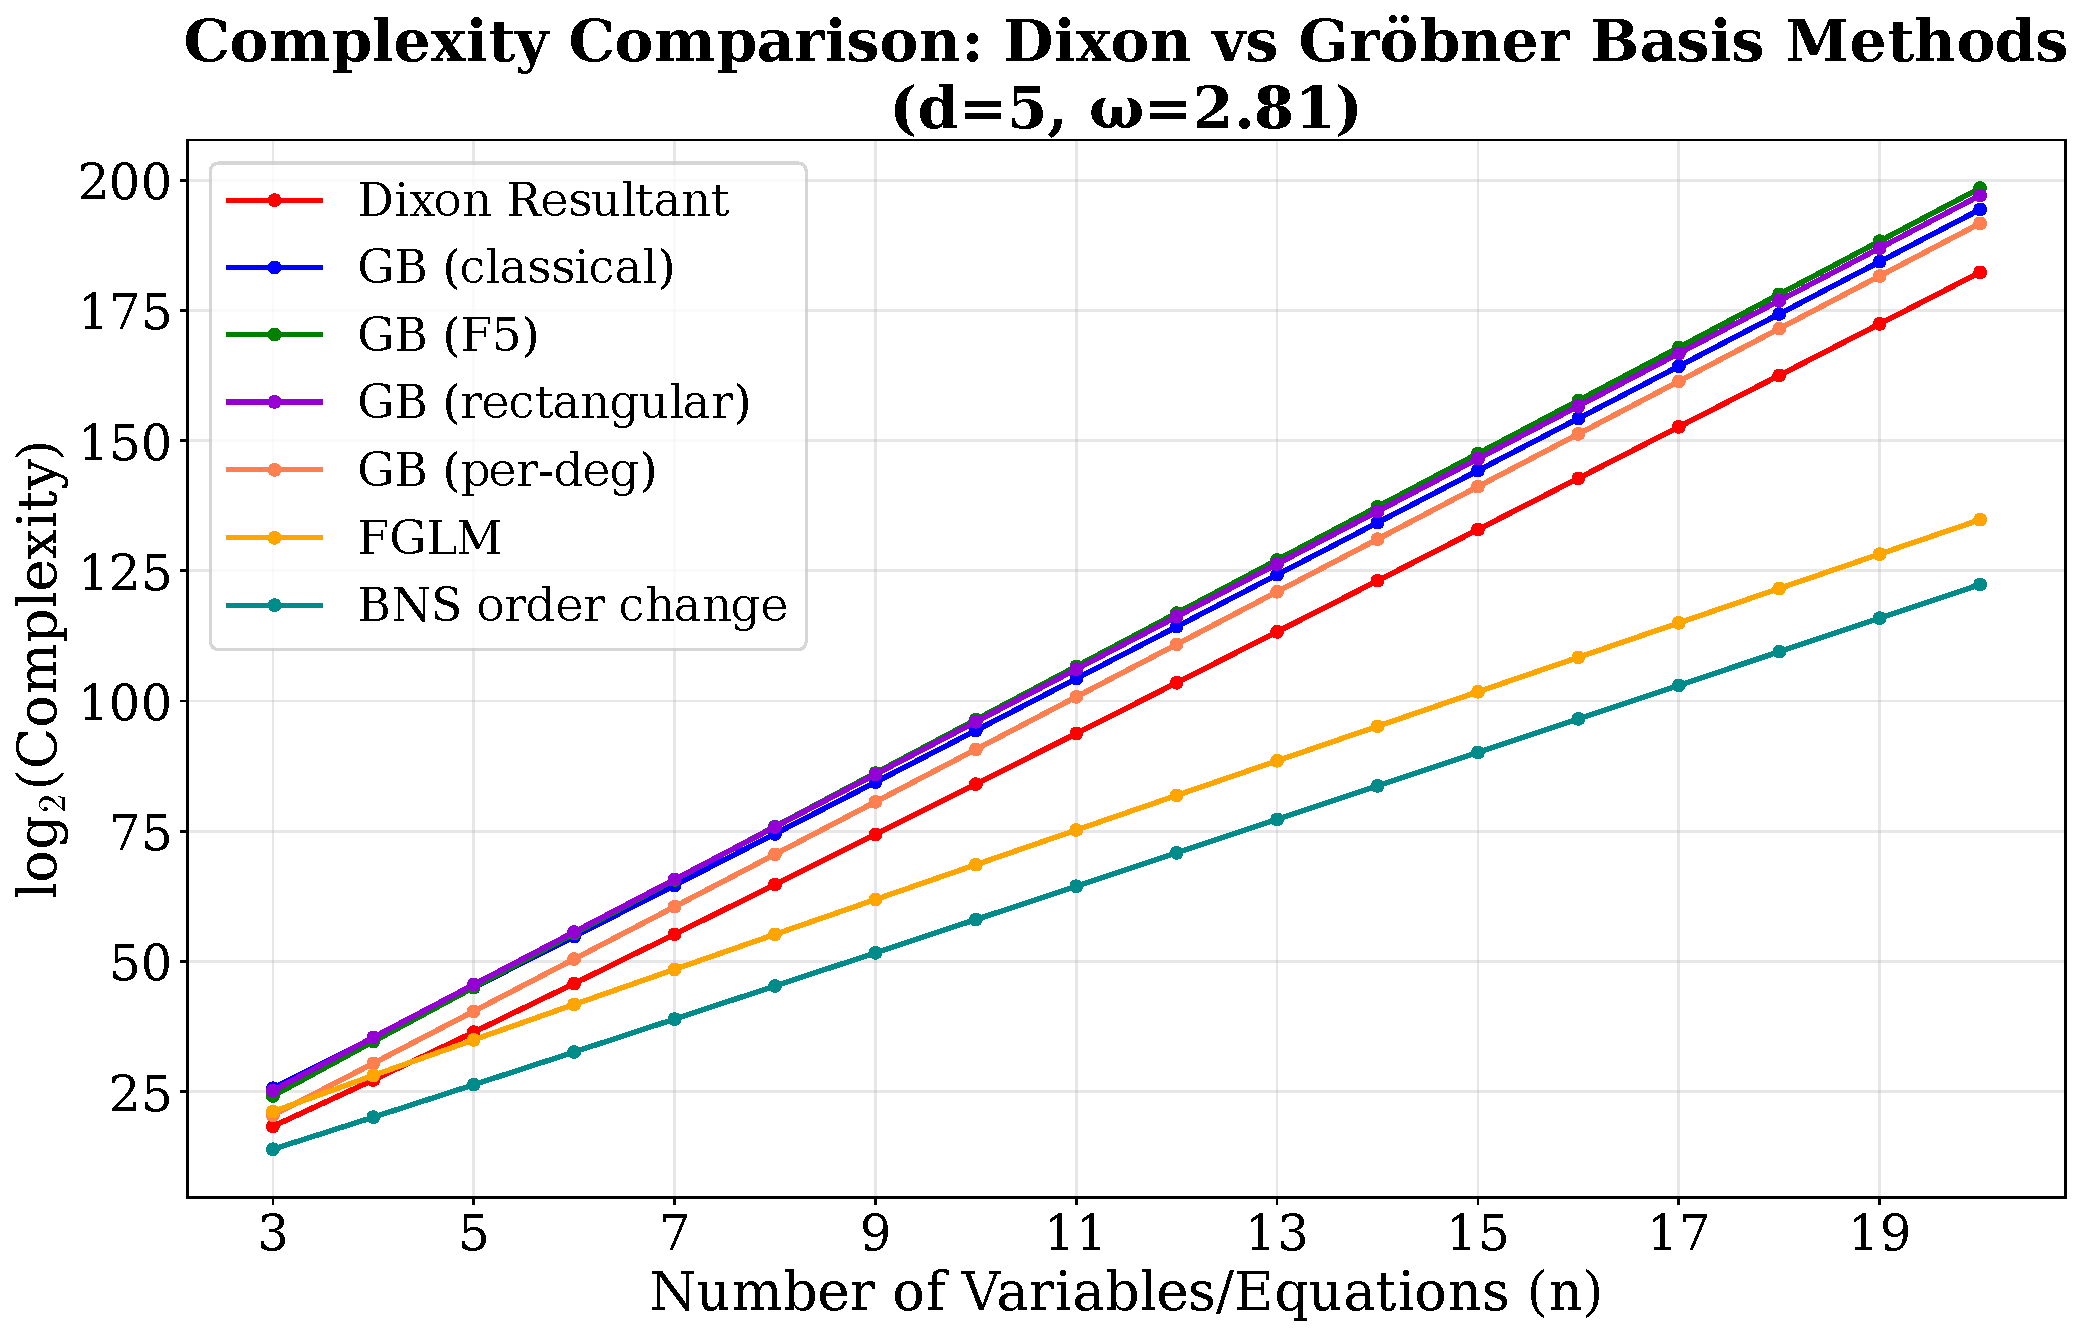
\includegraphics[width=0.85\textwidth]{complexity_comparison_d5.pdf}
	\par\smallskip\makebox[\textwidth][c]{(a)}\par
	\medskip
	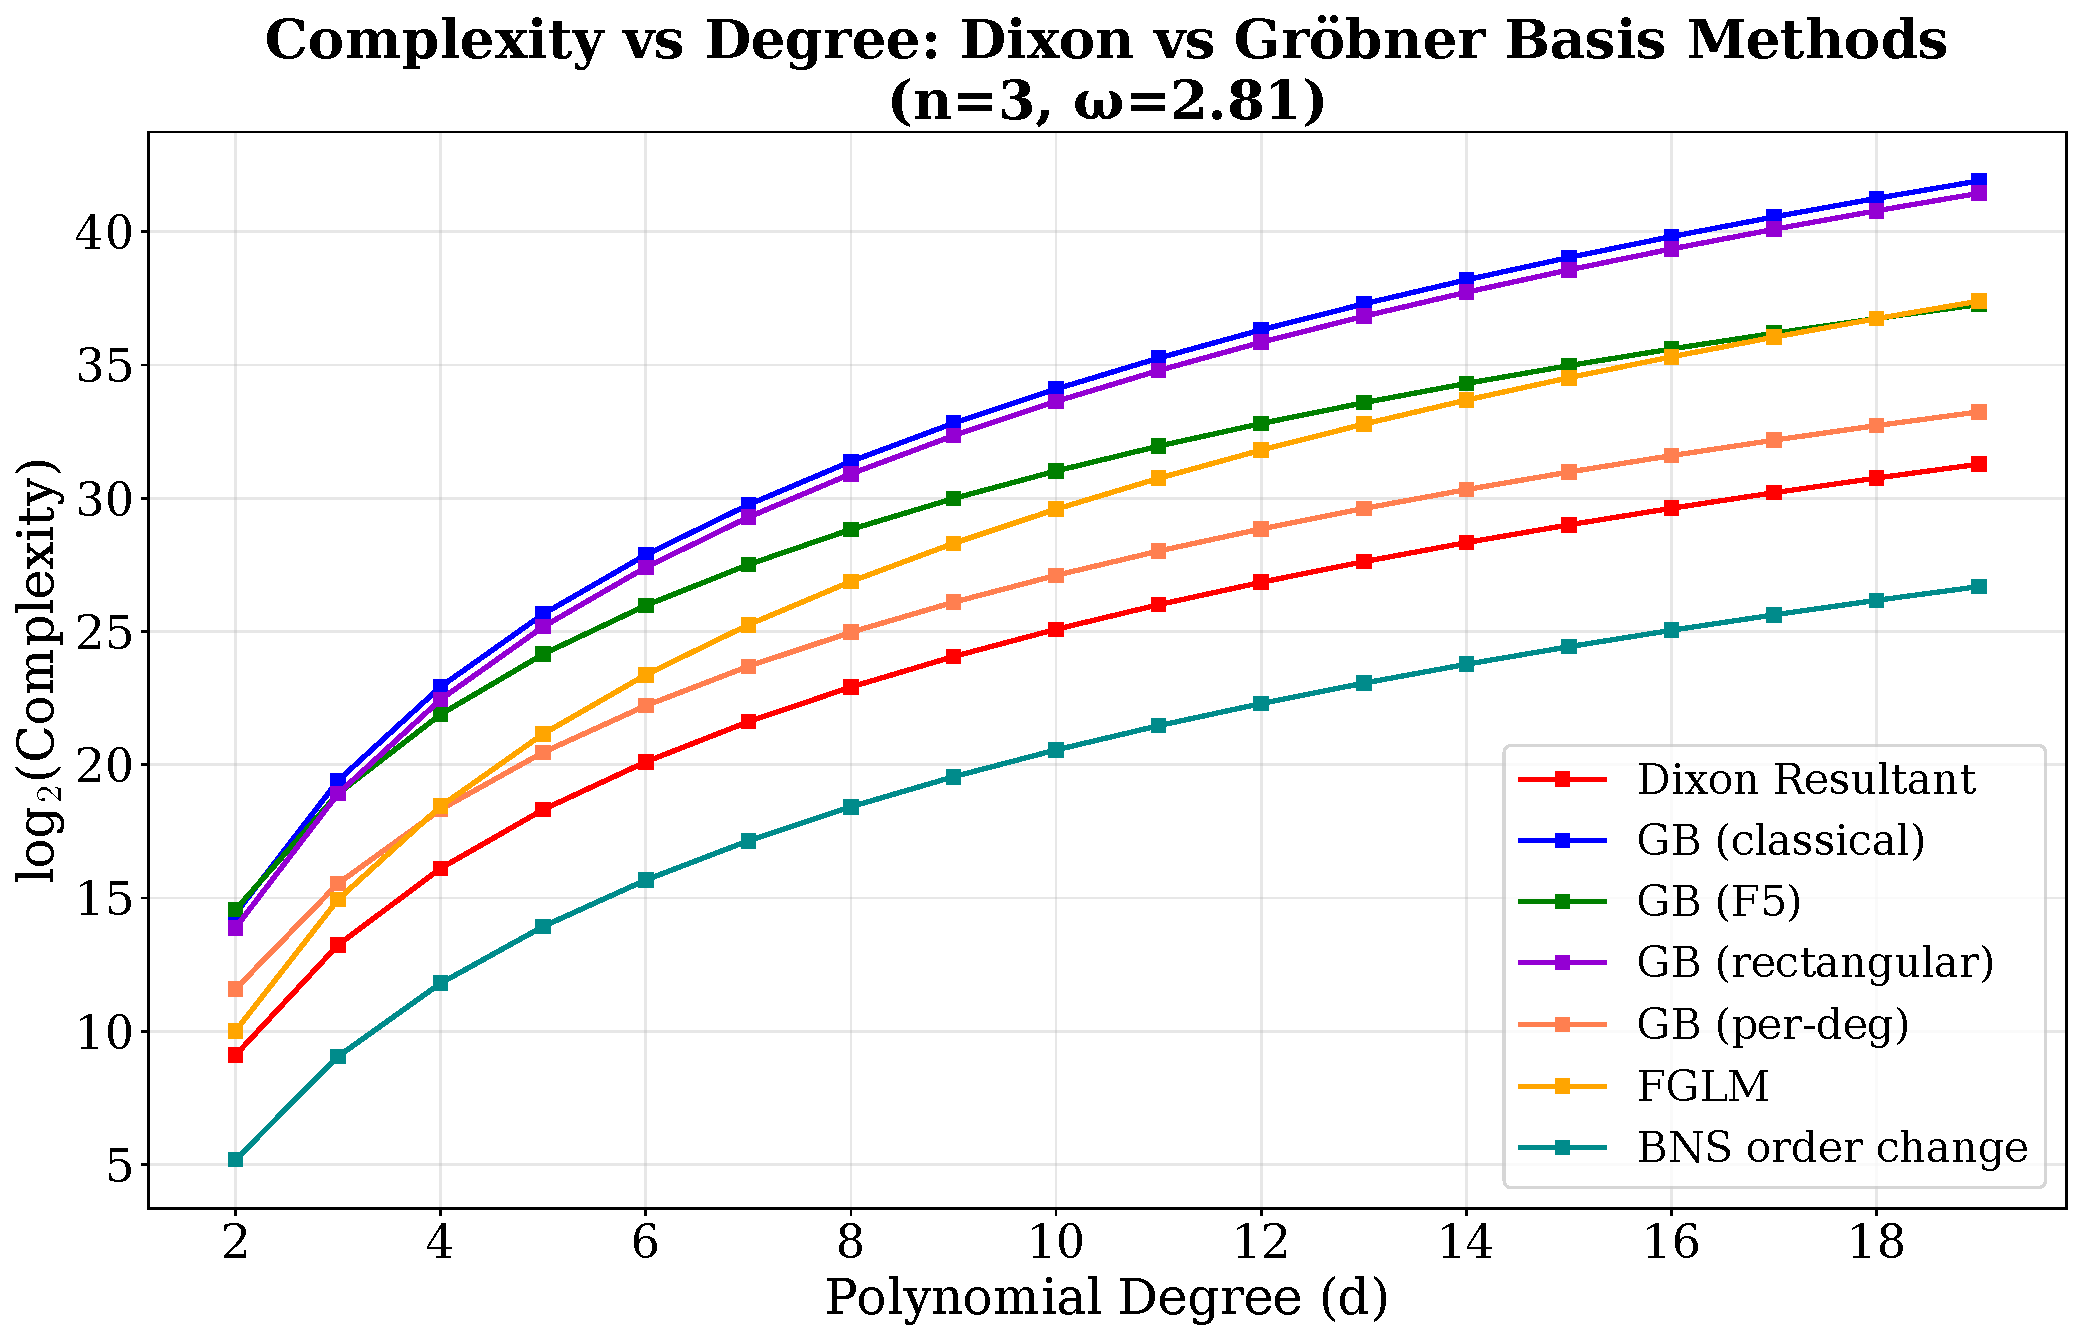
\includegraphics[width=0.85\textwidth]{complexity_vs_degree_n3.pdf}
	\par\smallskip\makebox[\textwidth][c]{(b)}\par
	\caption{Complexity comparison between the Dixon resultant and Gr\"obner basis}
	\label{fig:complexity}
\end{figure}
\begin{figure}[H]
	\centering
	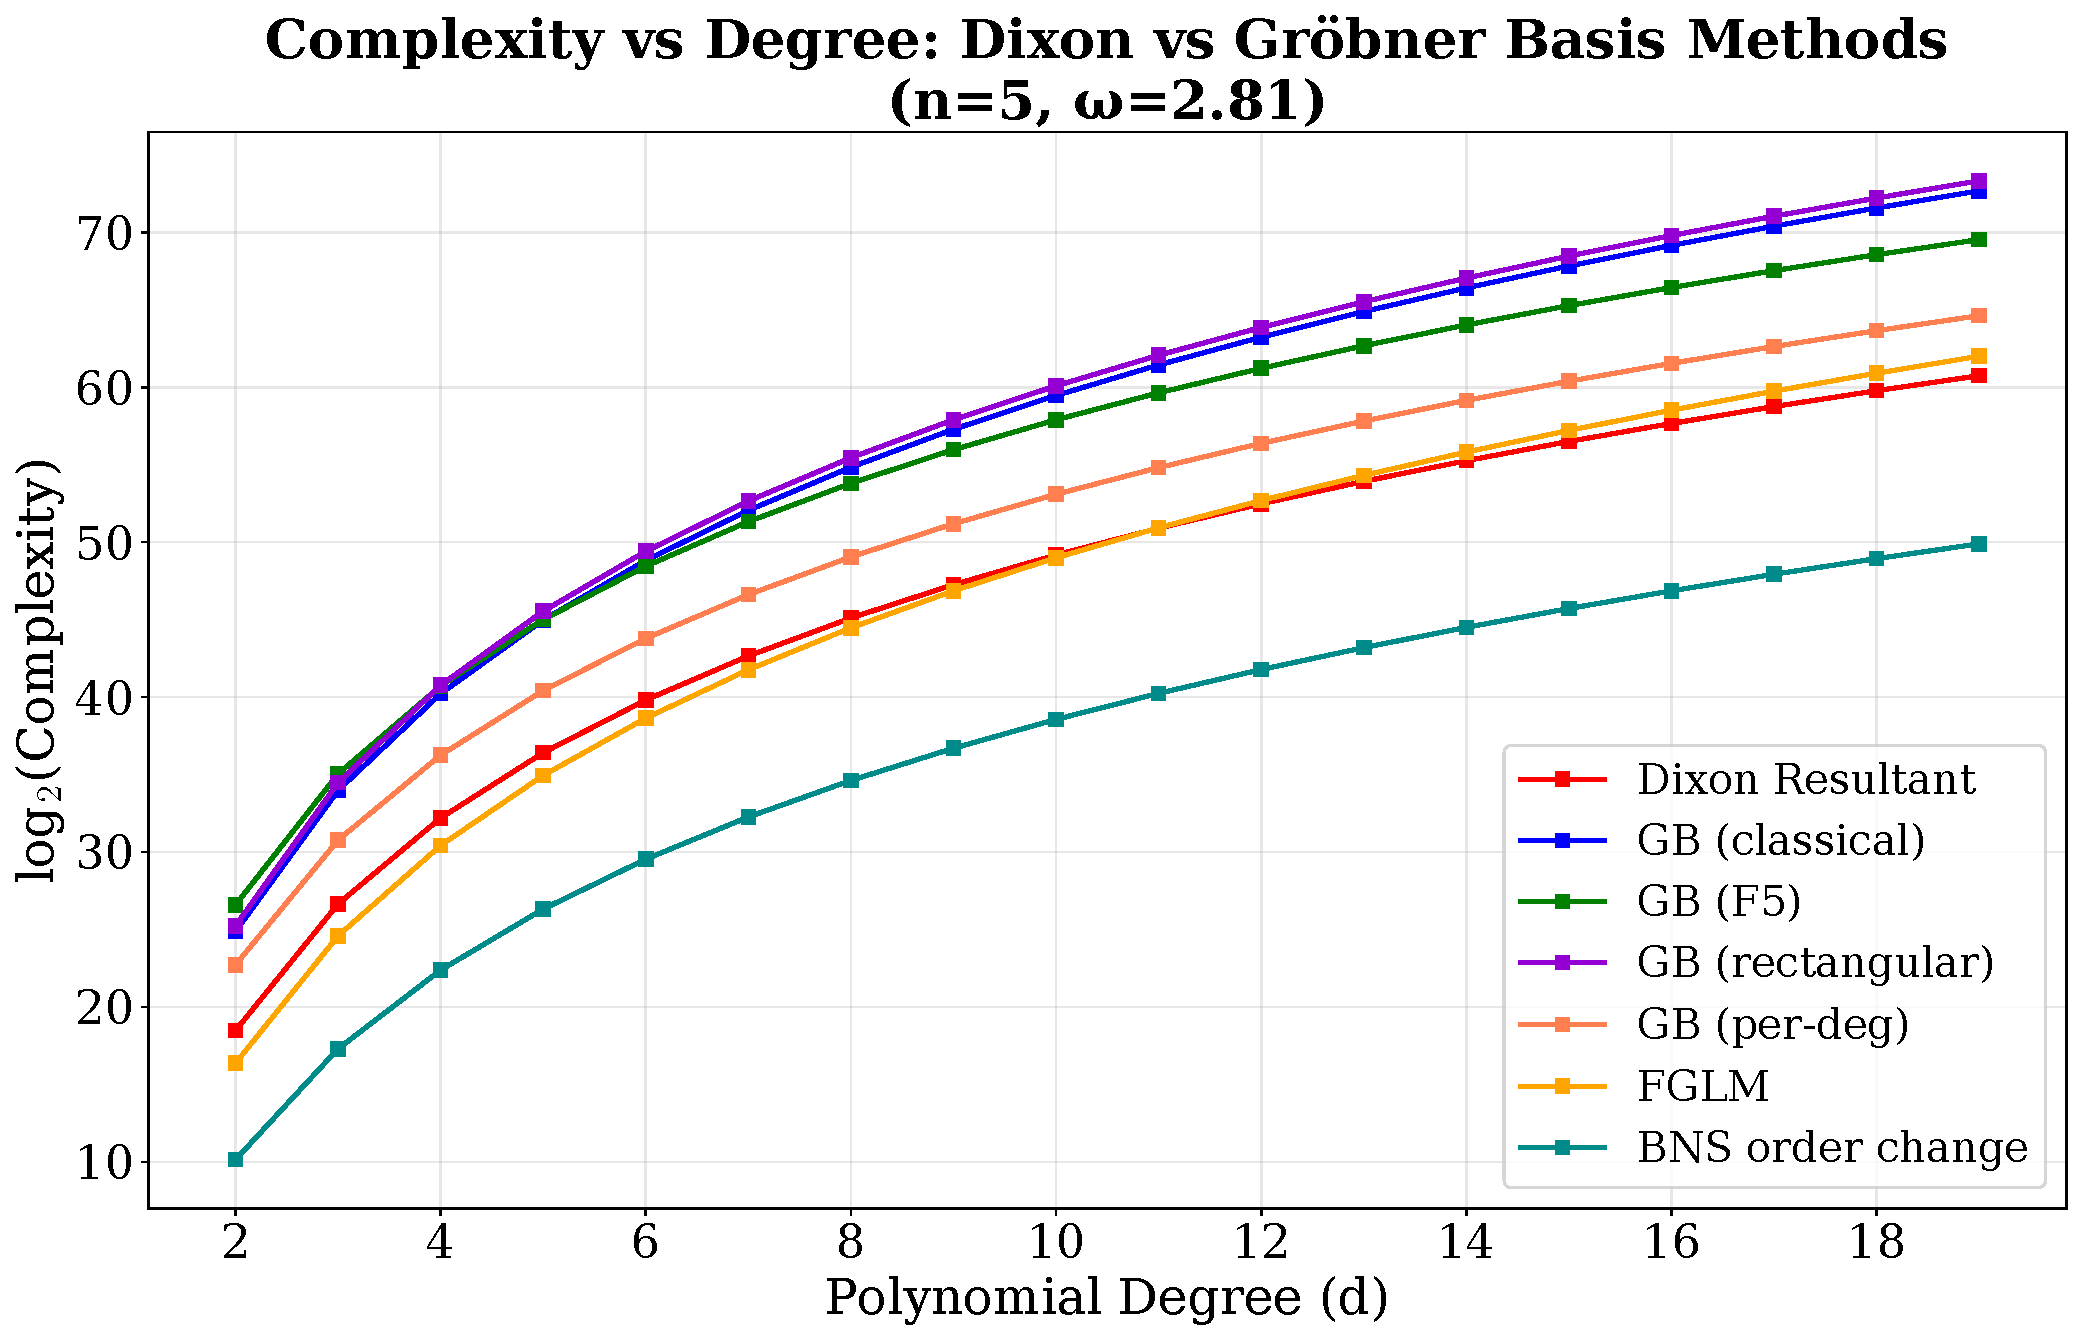
\includegraphics[width=0.85\textwidth]{complexity_vs_degree_n5.pdf}
	\par\smallskip\makebox[\textwidth][c]{(c)}\par
	\medskip
	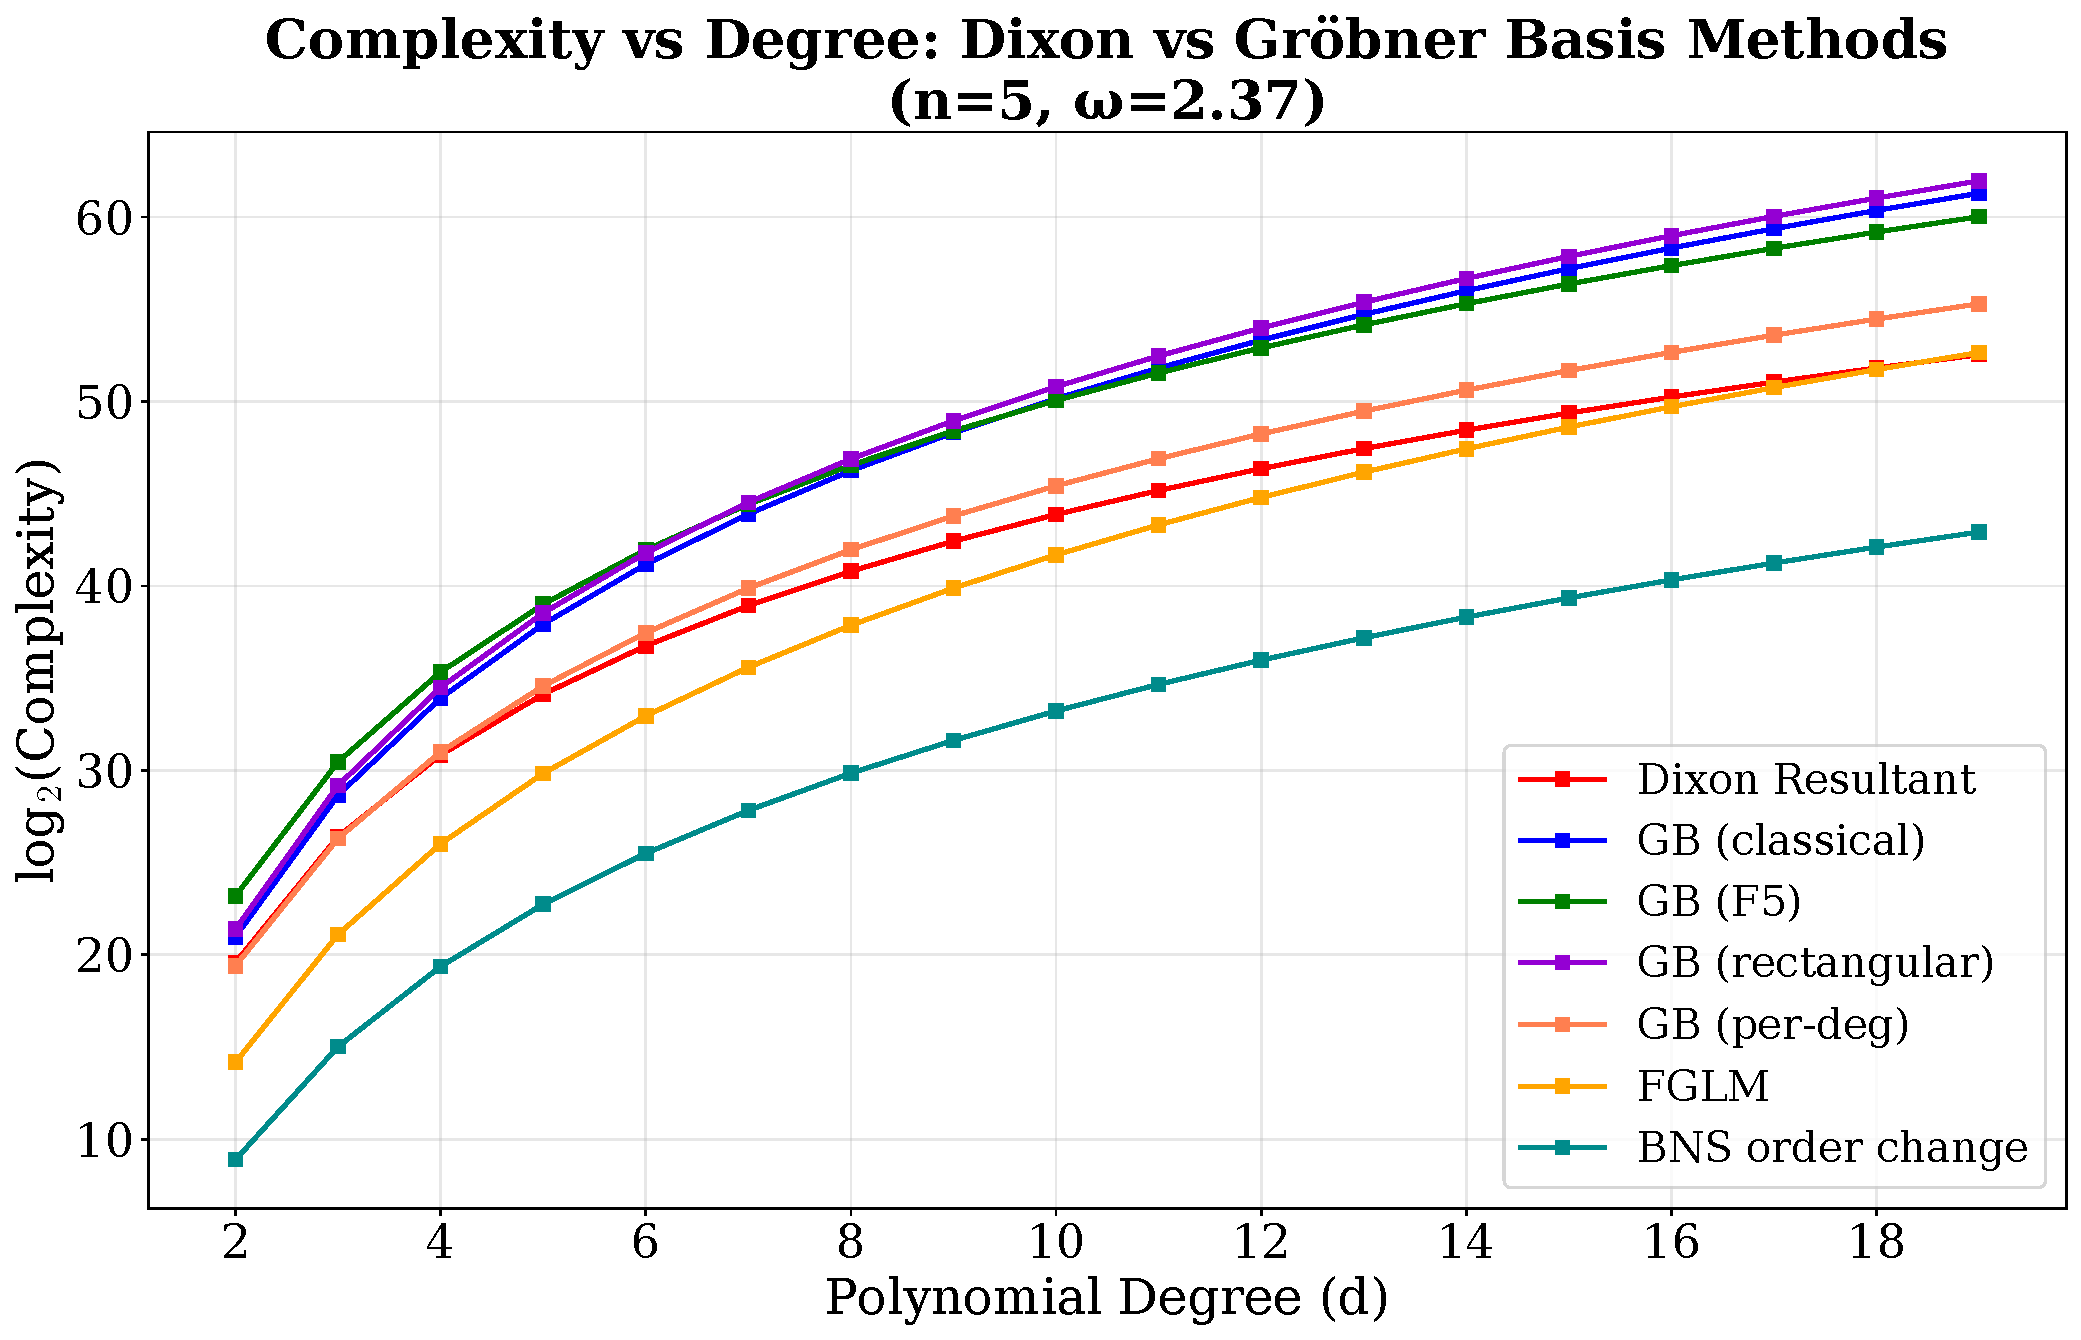
\includegraphics[width=0.85\textwidth]{complexity_vs_degree_n5w237.pdf}
	\par\smallskip\makebox[\textwidth][c]{(d)}\par
	\par\smallskip
	\begingroup\small\noindent
	\textbf{Fig.~\ref{fig:complexity} (continued).} Complexity comparison between the Dixon resultant and Gr\"obner basis.\par
	\endgroup
\end{figure}

\newpage
\section{Degree-Aware Submatrix Selection Algorithms}\label{appendix:algorithms}

Algorithm~\ref{alg:degree_optimal_selection} gives the pseudocode 
for the selection strategy described in Section~\ref{Subsection:Extraneous}.

\begin{algorithm}[htb!]
	\caption{Degree-aware maximal-rank submatrix selection}
	\label{alg:degree_optimal_selection}
	\begin{algorithmic}[1]
		\STATE \textbf{Input:} Polynomial matrix $\mathcal{M} \in \mathbb{K}[t_1, \ldots, t_m]^{r \times c}$ (possibly rectangular or rank-deficient)
		\STATE \textbf{Output:} Row indices $\mathcal{R}$ and column indices $\mathcal{C}$ with $|\mathcal{R}|=|\mathcal{C}|$ such that $\mathcal{M}(\alpha)[\mathcal{R}, \mathcal{C}]$ is nonsingular of order $\operatorname{rank}\mathcal{M}(\alpha)$, with selection guided by degree weights
		\STATE Initialize $\mathcal{R} \leftarrow \emptyset$, $\mathcal{C} \leftarrow \emptyset$
		\STATE Choose concrete evaluation point $\alpha = (\alpha_1, \ldots, \alpha_m) \in \mathbb{F}^m$
		\STATE Evaluate $\mathcal{M}_{\text{const}} \leftarrow \mathcal{M}(\alpha_1, \ldots, \alpha_m)$ \COMMENT{Constant matrix}
		\STATE Compute row degree weights: $d_r(i) \leftarrow \max_{j} \deg(\mathcal{M}_{i,j})$ for each row $i$
		\STATE Compute column degree weights: $d_c(j) \leftarrow \max_{i} \deg(\mathcal{M}_{i,j})$ for each column $j$
		\STATE Sort row indices by increasing degree weights: $\pi_r$
		\STATE Sort column indices by increasing degree weights: $\pi_c$
		
		\STATE Initialize basis tracker: $\mathcal{B} \leftarrow \emptyset$
		\FOR{each candidate index $k$ in $\pi_r$}
		\STATE Extract row vector $\vvec_k$ from $\mathcal{M}_{\text{const}}$
		\STATE Eliminate $\vvec_k$ against existing basis vectors in $\mathcal{B}$
		\IF{$\vvec_k \neq \mathbf{0}$ after elimination}
		\STATE Normalize $\vvec_k$ and add it to $\mathcal{B}$
		\STATE Include $k$ in $\mathcal{R}$
		\ENDIF
		\ENDFOR
		
		\STATE Reset basis tracker: $\mathcal{B} \leftarrow \emptyset$
		\FOR{each candidate index $k$ in $\pi_c$}
		\STATE Extract column vector $\vvec_k$ from $\mathcal{M}_{\text{const}}$
		\STATE Eliminate $\vvec_k$ against existing basis vectors in $\mathcal{B}$
		\IF{$\vvec_k \neq \mathbf{0}$ after elimination}
		\STATE Normalize $\vvec_k$ and add it to $\mathcal{B}$
		\STATE Include $k$ in $\mathcal{C}$
		\ENDIF
		\ENDFOR
		
		\RETURN $\mathcal{R}, \mathcal{C}$
	\end{algorithmic}
\end{algorithm}

The selected submatrix has the rank of the evaluated matrix; it has maximal polynomial-matrix rank when evaluation preserves rank. The degree weights guide the selection but do not guarantee a globally minimal determinant degree. After evaluation and weight computation, selection uses two Gaussian eliminations on constant matrices and sorting, within the bound in Equation~\eqref{eq:complexity_step3}. 


\newpage
\section{Experimental Results of Degree-Aware Submatrix Selection}\label{appendix:degree_optimal_exp}

We present the experimental results of Algorithm~\ref{alg:degree_optimal_selection} to assess Heuristic~\ref{hyp:bezout_attainment}. 
Table~\ref{tab:extraneous_factor_probability} compares the performance of our degree-aware selection strategy against naive random selection across various polynomial system configurations.

\begin{table}[htbp]
	\centering
	\caption{Frequency of B\'ezout-bound violations}
	\label{tab:extraneous_factor_probability}
	\begin{tabular}{cccccc}
		\hline
		\multirow{2}{*}{$n_x$} & \multirow{2}{*}{$k$} & Degrees & B\'ezout Bound & \multicolumn{2}{c}{B\'ezout violations} \\
		\cline{5-6}
		& & $(d_1,\ldots,d_{n_x+1})$ & $\prod d_i$ & Naive & Algorithm~\ref{alg:degree_optimal_selection} \\
		\hline
		2 & 1 & $(3,4,5)$ & 60 & 195/200 & 0/200 \\
		2 & 1 & $(5,6,6)$ & 180 & 200/200 & 0/200 \\
		2 & 1 & $(5,5,5)$ & 125 & 192/200 & 0/200 \\
		5 & 1 & $(2,2,2,2,2,2)$ & 64 & 199/200 & 0/200 \\
		3 & 2 & $(2,2,3,3)$ & 36 & 177/200 & 1/200 \\
		\hline
		\multicolumn{4}{c}{Observed violation frequency} & 963/1000 & 1/1000 \\
		\hline
	\end{tabular}
	
\end{table}

In Table~\ref{tab:extraneous_factor_probability}, $n_x$ denotes the number of variables to eliminate (so the system contains $n_x+1$ polynomials, consistent with the convention in the main text where $n$ is the number of polynomials),
$k$ denotes the number of parameters retained. We count cases with $\deg(\text{Res}(\mathcal{F})) > \prod d_i$; passing this test does not certify the absence of extraneous factors or excess multiplicities. The naive method uses random submatrix selection. All experiments were conducted over $\mathbb{F}_{65537}$ with 200 repetitions per system configuration. The observed violations for Algorithm~\ref{alg:degree_optimal_selection} exceeded the B\'ezout bound by at most $1$--$2$.

\newpage
\section{Detailed Stage-wise Complexity Parameters}\label{appendix:stage_details}

This appendix provides the detailed parameter derivations and the full set of five determinant models (expansion, Bareiss, Kronecker$+$HNF, interpolation, sparse) for the two symbolic-determinant stages whose preferred models were summarized in Section~\ref{Section:Estimate}. We keep the notation of Section~\ref{Section:Estimate} throughout: $\mathcal{F}$ is an $(n;d)$-system in $n-1+k$ variables, $C_n^{(d)}$ is the generic Dixon-matrix size, and we use the determinant-method complexity templates from Appendix~\ref{appendix:determinant_methods}.

\subsection{Step 1 Parameter Derivations}\label{appendix:step1}

This subsection derives the four abstract parameters $(\mu_1,S_1,L_1,\delta_1)$ and the additional grid-size parameter $N_1$ used to instantiate the five Step~1 complexity models. The expressions for $(\mu_1,S_1,L_1)$ recover~\eqref{eq:step1_params} in Section~\ref{Section:Estimate}, and substituting them into the determinant templates of Table~\ref{tab:determinant_methods} reproduces~\eqref{eq:step1_minor}--\eqref{eq:step1_sparse}.

The refined construction of the cancellation matrix from~\eqref{eq:Dixon_polynomial_improve} lowers several \emph{dual}-variable degrees by one through the difference quotients in $x_i-\bar{x}_i$, but this affects only the eliminated and dual variables and not the retained parameters $\avec$. For the asymptotic estimates below we use uniform upper bounds that are simpler to state. The determinant in Step~1 involves $\ell=2n+k-2$ variables (the $n-1$ original variables, the $n-1$ dual variables, and the $k$ retained parameters), with each entry having parameter total degree at most $d$. Summing across the $n$ rows of the determinant, the parameter total degree of $\det(\widehat{C})$ is therefore at most
\[
B_1 := \sum_{i=1}^{n} d = nd.
\]

\paragraph{Dense monomial-count proxy.}
The expansion-by-minors model uses the dense monomial-count proxy
\[
\mu_1 := \binom{n-1+k+d}{n-1+k},
\]
i.e.\ the number of dense monomials in the original $f_j$ when viewed as a polynomial in the $n-1+k$ variables of $\xvec$ and $\avec$ of total degree at most $d$. Explicitly expanding the difference-quotient entries would introduce a factor $\max\{1,d/(n+k)\}$ in the uniform entry-support bound. The theoretical expansion model avoids this factor by multiplying the undivided numerators of a difference-quotient row by the cached minors, summing the row expansion, and only then dividing exactly by the common linear factor $x_i-\bar{x}_i$. Each numerator has at most $2\mu_1$ terms, and this linear division is soft-linear in the input and output support sizes. By Lemma~\ref{lem:intermediate_support}, with $U:=S_1$, the cost therefore remains $\widetilde{O}(n2^n\mu_1S_1)$, as in~\eqref{eq:step1_minor}.

\paragraph{Variable-wise degree bounds.}
The Kronecker$+$HNF model uses the variable-wise degree bounds derived from the refined cancellation-matrix structure. A row-by-row analysis of $\widehat{C}$ (the variable $x_i$ appears in rows $1,\ldots,i$ with degree $\leq d$, in row $i+1$ with degree $\leq d-1$ after the difference quotient, and is absent from rows $i+2,\ldots,n$ where it has been replaced by $\bar{x}_i$; an analogous count applies to $\bar{x}_i$) gives
\[
\begin{aligned}
	b_{x_i} &:= \deg_{x_i}(\det\widehat{C})\le (i+1)d-1, &\quad
	b_{\bar{x}_i} &:= \deg_{\bar{x}_i}(\det\widehat{C})\le (n-i)d-1,\\
	b_{a_j} &:= \deg_{a_j}(\det\widehat{C})\le nd, &&
\end{aligned}
\]
for $i=1,\ldots,n-1$ and $j=1,\ldots,k$. Every entry has total degree at most $d$, so in particular $e_{x_i}, e_{\bar x_i}, e_{a_j}\le d$. Kronecker substitution must use the determinant-level base $b_*+1$ (per Appendix~\ref{appendix:determinant_methods}). For concreteness, let $b_1,\ldots,b_\ell$ denote the variable-wise determinant degrees in some fixed ordering of the $\ell=2n+k-2$ variables. The largest Kronecker weight is $\prod_{i=1}^{\ell-1}(b_i+1)$; using the entry total-degree bound, the average column degree of the univariate matrix is bounded by
\[
\delta_1 := d\cdot\prod_{i=1}^{\ell-1}(b_i+1)\;\le\;\prod_{i=1}^{\ell}(b_i+1),
\]
where $d$ is the total-degree bound of an entry and $d\le b_\ell+1$ for the structural bounds above. The estimate is valid for any fixed variable ordering, although its value may depend on that ordering. The HNF cost is then $T_{1}^{\mathrm{HNF}}=\widetilde{O}(n^\omega \delta_1)$.

\paragraph{Interpolation parameters.}
For evaluation-interpolation, the tensor-grid size is
\[
N_1=\prod_{i=1}^{2n+k-2}(b_i+1),
\]
and one probe evaluates the $n^2$ entries of $\widehat{C}$ at a point of $\mathbb{F}_q^{\ell}$ and computes the determinant of the resulting $n\times n$ constant matrix. Each entry $f_j$ is a polynomial in the $n-1+k$ variables of $\xvec,\avec$ with at most $\mu_1$ monomials, so building the evaluated matrix from $n$ underlying polynomials at $n$ points costs $\widetilde{O}(n^2\mu_1)$ field operations, and the constant determinant costs $\widetilde{O}(n^\omega)$. Therefore
\[
L_1 = \widetilde{O}(n^\omega + n^2\mu_1).
\]

\paragraph{Sparse term bound.}
The sparse model uses the structural term bound
\[
S_1 := \bigl(C_n^{(d)}\bigr)^2\binom{B_1+k}{k},
\]
where the factor $\bigl(C_n^{(d)}\bigr)^2$ comes from the bilinear Dixon support (each of $\xvec,\bar\xvec$ contributes at most $C_n^{(d)}$ distinct monomials by Lemma~\ref{lem:dixon_fc_bound}), and $\binom{B_1+k}{k}$ bounds the number of parameter monomials of total degree at most $B_1$ in the $k$ retained parameters $\avec$; see Appendix~\ref{appendix:determinant_methods} for the full derivation.

\paragraph{Intermediate minors.}
The same structural term bound controls all intermediate minors, not merely the final Dixon polynomial.
\begin{lemma}\label{lem:intermediate_support}
Let $n\ge2$, $d\ge2$, $k\ge1$, and $\deg_{\xvec,\avec}f_i\le d$.
Every square minor $H$ of $\widehat C$ satisfies
\[
 \#\operatorname{Supp}(H)
 \le\binom{nd+n+k-1}{2n+k-2}
 \le \bigl(C_n^{(d)}\bigr)^2\binom{nd+k}{k}=S_1.
\]
This holds over any field, without a genericity assumption.
\end{lemma}
\begin{proof}
The first row of $\widehat C$ has total degree at most $d$; every other row has degree at most $d-1$. Thus a $j$-row minor has degree at most $j(d-1)+1\le n(d-1)+1$ in $2n+k-2$ variables, giving the first inequality.
For the second, use $C_n^{(d)}=\binom{nd}{n-1}/n$ and put
\[
 R(n,m,k)=\frac{n^2\binom{m+n+k-1}{2n+k-2}}
 {\binom{m}{n-1}^2\binom{m+k}{k}},\qquad m\ge2n.
\]
The ratios
\[
 \frac{R(n,m,k+1)}{R(n,m,k)}
 =\frac{(m+n+k)(k+1)}{(2n+k-1)(m+k+1)}<1,
\]
\[
 \frac{R(n,m+1,1)}{R(n,m,1)}
 =1-\frac{n(n-1)}{(m+1)(m+2)}<1
\]
reduce the claim to $r_n:=R(n,2n,1)\le1$. Here $r_2=1$ and
\[
 \frac{r_{n+1}}{r_n}
 =\frac{(3n+1)(3n+2)(3n+3)(n+2)}
 {8n(2n+1)^2(2n+3)}\le1:
\]
the denominator minus numerator is
$(n-1)(37n^3+89n^2+60n+12)\ge0$.
Taking $m=nd$ proves the claim.\qed
\end{proof}
The bound concerns completed minors; temporary products in Bareiss updates may have $O(S_1^2)$ terms, as allowed by its cost model.

\paragraph{A division-free program for sparse interpolation.}
Huang's algorithm requires a division-free straight-line program (SLP), not only a scalar determinant black box~\cite[Definition~2 and Algorithm~9]{DBLP:journals/jsc/Huang23}.
A dense Horner program for $f_j$ has length $O(\mu_1)$. For two consecutive evaluations $A,B$ differing only in $x_i$, propagate the values and the divided difference $Q(h)=(h(A)-h(B))/(x_i-\bar x_i)$ through that program using
\[
 Q(u+v)=Q(u)+Q(v),\qquad
 Q(uv)=Q(u)v(A)+u(B)Q(v).
\]
The input differences are $0$ or $1$, so this computes each refined entry without division, including at $x_i=\bar x_i$. All entries cost $O(n^2\mu_1)$ operations. Composing with an $O(n^4)$ division-free determinant program~\cite{Rote2001DivisionFree} gives an SLP of length
\[
 O(n^2\mu_1+n^4)=O(n^2\mu_1),
\]
since $\mu_1\ge\binom{n+1}{2}$ for $d\ge2$.
Consequently Huang~\cite[Theorem~12]{DBLP:journals/jsc/Huang23} gives the stated expected sparse cost with Monte Carlo correctness. A sufficient characteristic condition is $p>nd$; any extension needed to obtain enough interpolation points is accounted for as in that theorem.

\paragraph{Step 1 complexity models.}
Substituting these parameters into the determinant models of Table~\ref{tab:determinant_methods} yields the following five Step~1 complexity estimates (all in field operations over $\mathbb{F}_q$):
\begin{align*}
	T_{1}^{\mathrm{minor}} &= \widetilde{O}(n2^n\mu_1S_1),\\
	T_{1}^{\mathrm{Bareiss}} &= \widetilde{O}(n^3S_1^2),\\
	T_{1}^{\mathrm{HNF}} &= \widetilde{O}(n^{\omega}\delta_1),\\
	T_{1}^{\mathrm{eval}} &= \widetilde{O}\!\left(N_1(L_1+\ell B_1)\right),\\
	T_{1}^{\mathrm{sparse}} &= \widetilde{O}(L_1S_1 + S_1\log q).
\end{align*}
In the expansion and Bareiss models, $U_1=S_1$ is justified by Lemma~\ref{lem:intermediate_support}; the cached-expansion formula uses the deferred linear division described above.

\paragraph{FDixon recursive construction.}
Besides the five determinant models, the direct recursive construction of Zhao and Fu~\cite{Zhao2005extfast} builds the Dixon matrix \emph{without} first forming the $n\times n$ cancellation determinant, so it replaces Steps~1 and~2 by a single block-recursive construction. Following the complexity model of Qin et al.~\cite[Theorem~3.1]{DBLP:journals/ijcm/QinWTJ17}, our implementation uses the surrogate
\[
T_{2}^{\mathrm{FDixon}}=\widetilde{O}\!\left(m_1^2\,(n!)^3\prod_{i=2}^{n}m_i^3\right),
\]
where the sorted surrogate degrees $m_i$ are the per-variable degree bounds selected in the code. (One can verify the $(n!)^3$ factor by combining the dominant term $n^3\cdot ((n-1)!)^3$ of~\cite[Eq.~(19)--(20)]{DBLP:journals/ijcm/QinWTJ17} with $n\cdot(n-1)!=n!$.) The factorial factor reflects the recursive enumeration of monomial supports inside the block recursion, which makes the estimate most attractive when $n$ is small and the degrees $m_i$ are large; for systems with many eliminated variables it becomes less competitive than the direct Step~1 path.

\subsection{Step 4 Parameter Derivations}\label{appendix:step4}

This subsection derives the abstract Step~4 parameters $(D_4,N_4,L_4,\delta_4,\mu_4,S_4)$ used to instantiate the five Step~4 complexity models. The expressions for $(D_4,N_4,L_4,\delta_4)$ recover~\eqref{eq:step4_params} in Section~\ref{Section:Estimate}, and substituting them into the determinant templates of Table~\ref{tab:determinant_methods} reproduces~\eqref{eq:step4_hnf}--\eqref{eq:step4_eval}.

Step~4 computes a symbolic determinant of a $C_n^{(d)}\times C_n^{(d)}$ polynomial matrix in the $k$ retained parameters $\avec$. Let $E_4\le nd$ be an entry-wise parameter-degree bound for the Step~4 matrix and $D_4\le d^{\,n}$ be the conditional B\'ezout total-degree bound for the determinantal output (Heuristic~\ref{hyp:bezout_attainment}).

\paragraph{Parameter expressions.}
A Kronecker base $C_n^{(d)}E_4+1$ suffices to avoid overflow in the encoded determinant; the resulting univariate matrix has average column degree bounded by
\[
\delta_4 := E_4 \prod_{j=1}^{k-1}(C_n^{(d)} E_4+1),
\]
which collapses to $\delta_4 = E_4 \le nd$ in the well-determined case $k=1$. The evaluation-interpolation and sparse-interpolation parameters are
\[
N_4 \le (D_4+1)^k,\qquad
S_4 \le \binom{D_4+k}{k},\qquad
L_4 = \widetilde{O}\!\left(\bigl(C_n^{(d)}\bigr)^\omega+\bigl(C_n^{(d)}\bigr)^2\mu_4\right).
\]
The dense monomial-count proxy for one matrix entry is
\[
\mu_4 := \binom{k+E_4}{k}.
\]

\paragraph{Intermediate-minor degree bound.}
The final degree bound $D_4$ does not by itself bound intermediate minors.
For the selected $\rho\times\rho$ matrix, let $a_{(1)}\le\cdots\le a_{(\rho)}$ and $b_{(1)}\le\cdots\le b_{(\rho)}$ be the sorted total degrees of its row and column monomial labels. Set $D_0=n(d-1)+1$. Since $\deg_{\avec}M_{uv}\le D_0-a_u-b_v$, every $j$-row minor has degree at most $jD_0-\sum_{i\le j}a_{(i)}-\sum_{i\le j}b_{(i)}$. Hence the certified choice
\begin{equation}\label{eq:step4_minor_support}
 H_4:=\max_{0\le j\le\rho}\left(jD_0-\sum_{i=1}^j a_{(i)}-\sum_{i=1}^j b_{(i)}\right),
 \qquad U_4:=\binom{H_4+k}{k}
\end{equation}
controls all intermediate minors. Without label information one may use $U_4=\binom{\rho E_4+k}{k}$. For mixed total degrees, replace $D_0$ by $\sum_i d_i-(n-1)$.

\paragraph{Probe cost and asymptotic effect.}
The term $C^2\mu_4$, with $C=C_n^{(d)}$, accounts for matrix evaluation. It also suffices for the entry-circuit part of a simultaneous value-and-gradient probe; the determinant part costs $\widetilde O(C^\omega)$ as explained in Appendix~\ref{appendix:sparse_oracle}.
Relative to the scalar determinant term, the added factor is $1+\mu_4/C^{\omega-2}$. For fixed $d,k$ and $\omega>2$, it tends to $1$ as $n\to\infty$. For fixed $n,k$ and $d\to\infty$, the ratio $\mu_4/C^{\omega-2}$ has order $d^{k-(n-1)(\omega-2)}$ when using $E_4=nd$. The HNF cost is unchanged.

\paragraph{Step 4 complexity models.}
The full set of five determinant models (all in field operations over $\mathbb{F}_q$) is:
\begin{align*}
	T_{4}^{\mathrm{minor}} &= \widetilde{O}\!\left(C_n^{(d)}2^{C_n^{(d)}}\mu_4U_4\right),\\
	T_{4}^{\mathrm{Bareiss}} &= \widetilde{O}\!\left(\bigl(C_n^{(d)}\bigr)^3U_4^2\right),\\
	T_{4}^{\mathrm{HNF}} &= \widetilde{O}\!\left(\bigl(C_n^{(d)}\bigr)^{\omega}\delta_4\right),\\
	T_{4}^{\mathrm{eval}} &= \widetilde{O}\!\left(N_4(L_4+kD_4)\right),\\
	T_{4}^{\mathrm{sparse}} &= \widetilde{O}(L_4S_4 + S_4\log q).
\end{align*}

\paragraph{Full table of stage-wise models.}
Table~\ref{tab:step14_models_full} collects all the formulas above.

\begin{table}[!htbp]
	\centering
	\small
	\caption{Complexity models instantiated for the first and final symbolic determinants.}
	\label{tab:step14_models_full}
	\setlength{\tabcolsep}{4pt}
	\renewcommand{\arraystretch}{1.05}
	\begin{tabular}{p{0.18\textwidth}p{0.34\textwidth}p{0.34\textwidth}}
		\toprule
		\textbf{Method} & \textbf{Step 1/2} & \textbf{Step 4} \\
		\midrule
		Expansion & $\widetilde{O}(n2^n\mu_1S_1)$ & $\widetilde{O}\!\left(C_n^{(d)}2^{C_n^{(d)}}\mu_4U_4\right)$ \\
		Bareiss & $\widetilde{O}(n^3S_1^2)$ & $\widetilde{O}\!\left(\bigl(C_n^{(d)}\bigr)^3U_4^2\right)$ \\
		Kronecker & $\widetilde{O}(n^\omega \delta_1)$ & $\widetilde{O}\!\left(\bigl(C_n^{(d)}\bigr)^\omega\delta_4\right)$ \\
		Interpolation & $\widetilde{O}(N_1(L_1+\ell B_1))$ & $\widetilde{O}(N_4(L_4+kD_4))$ \\
		Sparse & $\widetilde{O}(L_1S_1+S_1\log q)$ & $\widetilde{O}(L_4S_4+S_4\log q)$ \\
		FDixon & $\widetilde{O}(m_1^2(n!)^3\prod_{i=2}^{n}m_i^3)$ & --- \\
		\bottomrule
	\end{tabular}
\end{table}

\subsection{Step 1 vs Step 4 Comparison}\label{appendix:step_comparison}

This subsection gives the detailed comparison behind the main-text statement that the symbolic cost is usually governed by the final determinant computation. We first compare the most favorable first-determinant estimate with the univariate HNF model for the final determinant, and then relate this theoretical picture to the trend plots used in the paper.

\paragraph{Notation.}
We keep the notation of Section~\ref{Section:Estimate} and the preceding subsections. In particular, the first determinant is modeled by
\[
T_{1}^{\mathrm{minor}},\quad
T_{1}^{\mathrm{Bareiss}},\quad
T_{1}^{\mathrm{HNF}},\quad
T_{1}^{\mathrm{eval}},\quad
T_{1}^{\mathrm{sparse}},\quad
T_{2}^{\mathrm{FDixon}},
\]
while the final determinant is modeled by
\[
T_{4}^{\mathrm{minor}},\quad
T_{4}^{\mathrm{Bareiss}},\quad
T_{4}^{\mathrm{HNF}},\quad
T_{4}^{\mathrm{eval}},\quad
T_{4}^{\mathrm{sparse}}.
\]

\paragraph{Fixed degree.}
For $k=1$, fixed $d\ge2$, and $\omega>2$, sparse construction is asymptotically below the Step~4 HNF bound under the characteristic condition of Appendix~\ref{appendix:step1}. Cached expansion additionally requires~\eqref{eq:minor_threshold}. Appendix~\ref{appendix:wellsq} gives both ratios and the $\omega=2$ boundary case.

\paragraph{Comparison of $T_{1}^{\mathrm{HNF}}$ and $T_{4}^{\mathrm{HNF}}$ as $d$ grows.}
Fix $n$ and again take $k=1$. The variable-wise determinant degrees in the first determinant satisfy $b_i=\Theta(nd)$, with $\ell=2n-1$, and per-entry degree $\Theta(d)$, so (treating $n$ as fixed and letting $d\to\infty$)
\[
\delta_1 = d\cdot \prod_{i=1}^{\ell-1}(b_i+1) =\Theta(d^{2n-1}),
\qquad
T_{1}^{\mathrm{HNF}}=\widetilde{O}(n^\omega d^{2n-1}).
\]
For the final determinant,
\[
C_n^{(d)}=\Theta(d^{n-1}),
\qquad
T_{4}^{\mathrm{HNF}}=\widetilde{O}\!\left(nd\,\bigl(C_n^{(d)}\bigr)^\omega\right)=\widetilde{O}(d^{\omega(n-1)+1}).
\]
Since $\omega>2$, we have $\omega(n-1)+1>2n-1$ for every $n\ge 2$. Thus, for fixed $n$, the HNF complexity estimate for Step~4 has a strictly larger exponent in $d$ than that for Step~1. At the boundary $\omega=2$, the exponents coincide, so this comparison alone does not establish which stage dominates; the suppressed polylogarithmic factors and constants may affect their relative costs. In particular, the constants may depend strongly on $n$, which is held fixed in this analysis. For $\omega>2$, the comparison supports using Step~4 as the asymptotic bottleneck within the HNF model in the fixed-$n$, high-degree regime. This is consistent with our experiments, in which the final symbolic determinant dominates the running time. We treat $\omega=2$ as an idealized boundary used for the uniform-exponent security comparisons.

For any fixed $k\ge1$, the same comparison of construction and HNF bounds holds: at fixed $d$, sparse construction is $C^2\operatorname{poly}(n)$ while HNF is $C^{\omega+k-1}\operatorname{poly}(n)$. At fixed $n$, the respective Kronecker/HNF degree exponents are $2n+k-2$ and $(\omega+k-1)(n-1)+k$, differing by $(\omega+k-3)(n-1)>0$. The Step~4 interpolation bounds also grow faster than the corresponding construction bounds in these two regimes, under their output-degree hypotheses. These are comparisons of displayed bounds, not claims about the actual rank or running time. When sparse interpolation is unavailable, cached expansion requires the threshold~\eqref{eq:minor_threshold} in the fixed-$d$ regime.

\paragraph{Overall comparison.}
Construction is controlled by Kronecker$+$HNF in the fixed-$n$, high-degree regime, and by sparse interpolation or cached expansion in the fixed-$d$ regime under the conditions above. These comparisons are asymptotic; at moderate parameters the overall estimate retains both stages. Figures~\ref{fig:step14_vs_degree} and~\ref{fig:step14_vs_variables} show the individual cost models.

\begin{figure}[!htbp]
	\centering
	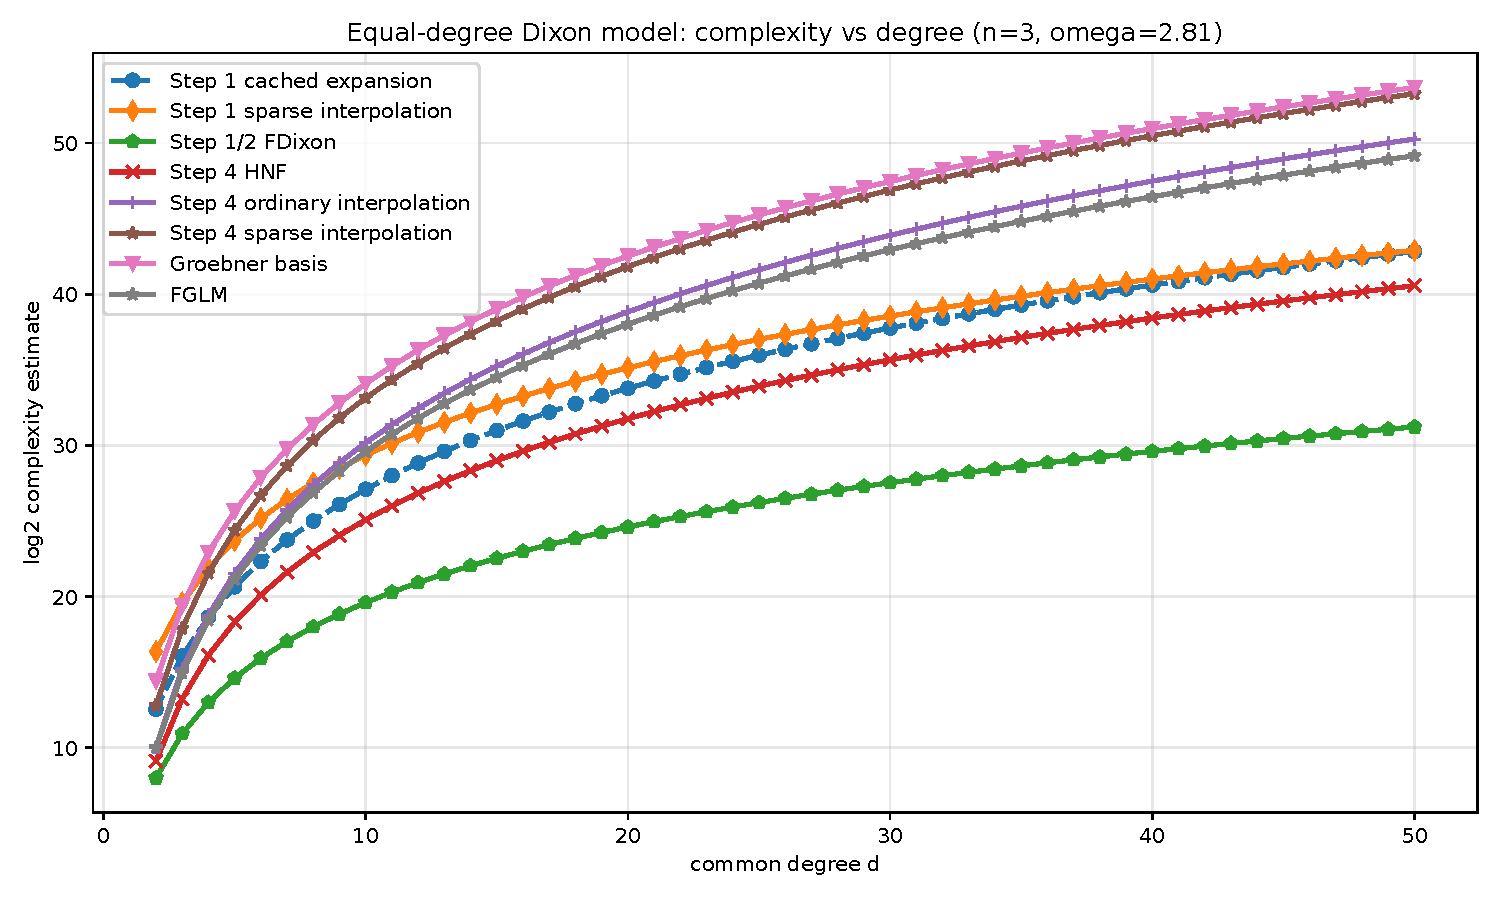
\includegraphics[width=0.92\textwidth]{plot_step1_step4_vs_degree.pdf}
	\caption{Comparison of the first and final determinant costs as the polynomial degree varies. The curves show the displayed cost models for $n=3$ and $k=1$.}
	\label{fig:step14_vs_degree}
\end{figure}

\begin{figure}[!htbp]
	\centering
	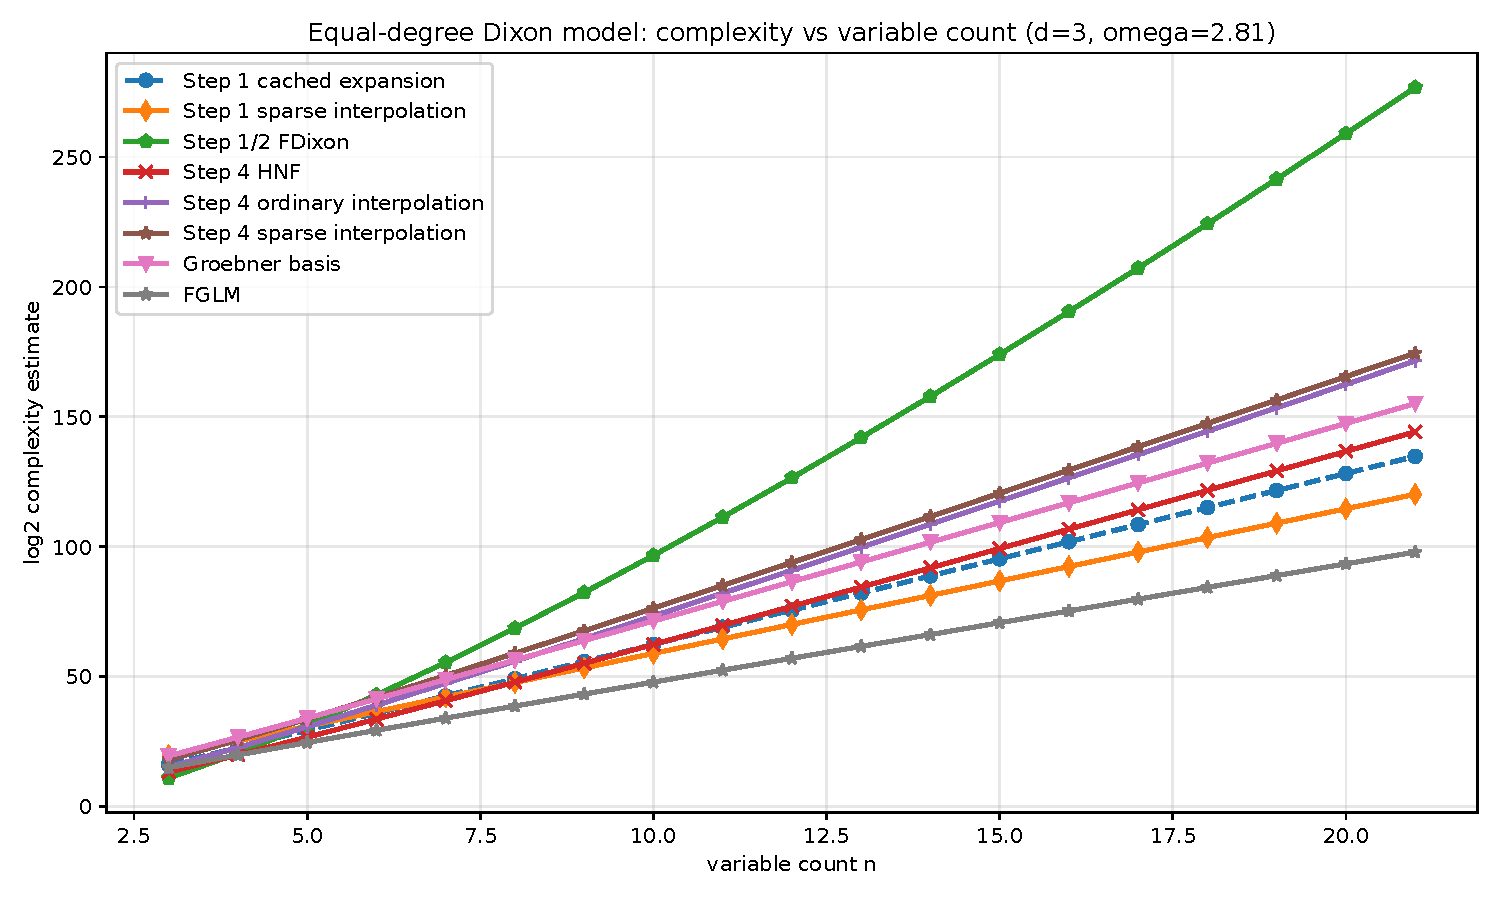
\includegraphics[width=0.92\textwidth]{plot_step1_step4_vs_variables.pdf}
	\caption{Comparison of the first and final determinant costs as the number of variables varies ($k=1$). The sparse curve assumes sufficiently large characteristic; cached expansion obeys the threshold~\eqref{eq:minor_threshold}.}
	\label{fig:step14_vs_variables}
\end{figure}

\subsection{Well-determined Case (\texorpdfstring{$k=1$}{k=1})}\label{appendix:wellsq}

We now specialize the comparison in Appendix~\ref{appendix:step_comparison} to the well-determined setting $k=1$, which is the case used both in the comparison with Gr\"obner basis methods (Section~\ref{Subsection:Other_Comparison}) and in the AO applications of Section~\ref{Section:Application}. The argument is more explicit than the general case because the parameter space is one-dimensional, so $D_4\le d^{\,n}$, $E_4\le nd$, $\delta_4=nd$, and Kronecker$+$HNF reduces to a single univariate HNF on a $C_n^{(d)}\times C_n^{(d)}$ matrix.

\paragraph{Explicit formulas.}
Substituting $k=1$ into the Step~1 and Step~4 templates of Appendices~\ref{appendix:step1} and~\ref{appendix:step4} gives
\begin{align}
	T_{4}^{\mathrm{HNF}}
	&= \widetilde{O}\!\left(nd\,\bigl(C_n^{(d)}\bigr)^\omega\right),
	\label{eq:wellsq_T4HNF}\\[0.3em]
	T_{1}^{\mathrm{sparse}}
	&= \widetilde{O}\!\bigl(n^2\,(nd+1)\binom{n+d}{n}\bigl(C_n^{(d)}\bigr)^2\bigr)
	= \widetilde{O}\!\bigl(n^3\,d\,\binom{n+d}{n}\bigl(C_n^{(d)}\bigr)^2\bigr),
	\label{eq:wellsq_T1sparse}\\[0.3em]
	T_{1}^{\mathrm{minor}}
	&= \widetilde{O}\!\bigl(n\,2^n(nd+1)\binom{n+d}{n}\bigl(C_n^{(d)}\bigr)^2\bigr)
	= \widetilde{O}\!\bigl(n^2 d\,2^n\binom{n+d}{n}\bigl(C_n^{(d)}\bigr)^2\bigr),
	\label{eq:wellsq_T1minor}
\end{align}
\paragraph{Asymptotic size of $C_n^{(d)}$.}
For fixed $d\ge 2$ and $n\to\infty$, the Fuss--Catalan formula and Stirling's approximation give
\begin{equation}\label{eq:fc_stirling}
	C_n^{(d)} \;=\; \frac{1}{n(d-1)+1}\binom{nd}{n}
	\;=\; \Theta\!\Bigl(\frac{\gamma_d^{\,n}}{n^{3/2}}\Bigr),
	\qquad
	\gamma_d := \frac{d^d}{(d-1)^{d-1}},
\end{equation}
where $\gamma_d>1$ for $d\ge 2$. The sequence $(\gamma_d)_{d\ge 2}$ is strictly increasing, with minimum $\gamma_2=4$, and grows like $\gamma_d\sim e\,d$ as $d\to\infty$. Equation~\eqref{eq:fc_stirling} shows that $C_n^{(d)}$ grows exponentially in $n$ for any fixed $d\ge 2$, while $\binom{n+d}{n}=\Theta(n^d)$ is only polynomial in $n$ for fixed $d$. This separation is the key quantitative input for the two comparisons below.

\paragraph{Comparison of $T_{4}^{\mathrm{HNF}}$ with $T_{1}^{\mathrm{sparse}}$.}
Forming the ratio and cancelling the common $d$-factors gives
\begin{equation}\label{eq:ratio_4HNF_1sparse}
	\frac{T_{4}^{\mathrm{HNF}}}{T_{1}^{\mathrm{sparse}}}
	\;=\; \widetilde{\Theta}\!\left(
	\frac{\bigl(C_n^{(d)}\bigr)^{\omega-2}}{n^2\,\binom{n+d}{n}}
	\right).
\end{equation}
Substituting~\eqref{eq:fc_stirling}, the numerator $\bigl(C_n^{(d)}\bigr)^{\omega-2}$ equals $\gamma_d^{\,(\omega-2)n}/n^{3(\omega-2)/2}$, which grows \emph{exponentially} in $n$ as long as $\gamma_d^{\,\omega-2}>1$, i.e.\ as long as $\omega>2$ (since $\gamma_d>1$ for $d\ge 2$). The denominator is polynomial in $n$ for fixed $d$. Hence for every $\omega>2$ and every fixed $d\ge 2$, the ratio~\eqref{eq:ratio_4HNF_1sparse} tends to infinity as $n\to\infty$, so
\[
T_{4}^{\mathrm{HNF}} \;\gg\; T_{1}^{\mathrm{sparse}}\quad\text{asymptotically in }n.
\]

\paragraph{Comparison of $T_{4}^{\mathrm{HNF}}$ with $T_{1}^{\mathrm{minor}}$.}
The same cancellation yields
\begin{equation}\label{eq:ratio_4HNF_1minor}
	\frac{T_{4}^{\mathrm{HNF}}}{T_{1}^{\mathrm{minor}}}
	\;=\; \widetilde{\Theta}\!\left(
	\frac{\bigl(C_n^{(d)}\bigr)^{\omega-2}}{n\,2^n\binom{n+d}{n}}
	\right)
	\;=\; \widetilde{\Theta}\!\left(
	\frac{(\gamma_d^{\,\omega-2}/2)^{\,n}}{\operatorname{poly}(n,d)}
	\right).
\end{equation}
This ratio tends to infinity as $n\to\infty$ \emph{iff} the base satisfies
\begin{equation}\label{eq:minor_threshold}
	\gamma_d^{\,\omega-2}>2,
	\qquad\text{equivalently}\qquad
	\omega \;>\; 2+\frac{\log 2}{\log \gamma_d}.
\end{equation}
The right-hand side of~\eqref{eq:minor_threshold} is strictly decreasing in $d$: for $d=2$ it equals $2+\tfrac{\log 2}{\log 4}=2.5$; for $d=3$ it equals $2+\tfrac{\log 2}{\log(27/4)}\approx 2.363$; and it tends to $2$ from above as $d\to\infty$. In particular, for the Strassen exponent $\omega\approx 2.81$ used in our timing tables and Sections~\ref{Section:Application}--\ref{Subsection:Other_Comparison}, condition~\eqref{eq:minor_threshold} is met for all $d\ge 2$ (e.g.\ $\gamma_2^{0.81}\approx 3.07>2$). Hence
\[
T_{4}^{\mathrm{HNF}} \;\gg\; T_{1}^{\mathrm{minor}}\quad\text{asymptotically in }n,
\]
for every $\omega\ge 2.81$ and every $d\ge 2$ (and more generally whenever~\eqref{eq:minor_threshold} holds).

\paragraph{Boundary case $\omega=2$.}
For fixed $d$ and $\omega=2$, equations~\eqref{eq:ratio_4HNF_1sparse} and~\eqref{eq:ratio_4HNF_1minor} give ratios of order $1/(n^2\binom{n+d}{n})$ and $1/(n2^n\binom{n+d}{n})$, respectively, up to logarithmic factors. Thus these two construction bounds exceed the HNF bound for Step~4 as $n$ grows; cached expansion retains its additional $2^n$ factor. The value $\omega=2$ is used for the uniform-exponent comparison in \vision, where the overall estimate takes the maximum over all stages (Appendix~\ref{appendix:vision}). For $\omega>2$, the sparse comparison and the cached-expansion threshold~\eqref{eq:minor_threshold} apply under their stated hypotheses.

\newpage
\section{Alternative Determinant Computation Methods}\label{appendix:determinant_methods}

This appendix expands the determinant-method summary from Table~\ref{tab:determinant_methods}. We record both the complexity formulas and the stage-specific origin of the parameters used in the comparison code.

\paragraph{Notation.}
Let $P(\yvec)$ be an $m\times m$ polynomial matrix in variables $\yvec=(y_1,\ldots,y_v)$. Let $b_i$ bound the degree of $\det(P)$ in $y_i$ (this determines the Kronecker substitution base, which must avoid overflow), and let $e_i\le b_i$ bound the degree of a single entry of $P$ in $y_i$. With $c_i=\prod_{j<i}(b_j+1)$, define
\[
\delta = \sum_{i=1}^{v}e_i c_i,
\qquad
N = \prod_{i=1}^{v}(b_i+1),
\]
where $\delta$ bounds the entry degree, hence the average column degree, of the univariate matrix obtained after Kronecker substitution. Since $\sum_{i<v}b_i c_i=c_v-1$, we have $\delta\le(e_v+1)c_v-1<2e_vc_v$ when $e_v\ge1$; this yields the asymptotic cost $\widetilde{O}(m^\omega e_vc_v)$. If every entry has total degree at most $E$, the bound $\delta=Ec_v$ may be used instead. This gives the Step~1 and Step~4 specializations with $E=d$ and $E=E_4\le nd$, respectively.
We also write $B:=\max_i b_i$, $L$ for the cost of one determinant probe, $S$ for a sparsity bound on $\det(P)$, $U$ for an upper bound on the support size of intermediate minors arising during a chosen evaluation strategy, $\mu$ for a dense monomial-count bound on one entry of $P$, and $\widetilde{M}(u)$ for soft-Oh multiplication at degree $u$.

\paragraph{Intermediate-minor support bounds.}
The output support bound $S$ and the intermediate-minor bound $U$ serve different purposes. For Step~1, Lemma~\ref{lem:intermediate_support} proves $U_1=S_1$ is valid for the uniform total-degree setting. For Step~4, use~\eqref{eq:step4_minor_support}, or the coarser dense degree bound stated there; a bound on the final determinant degree alone does not justify $U_4=S_4$.

\subsection{Expansion}
A baseline model is expansion by minors~\cite{GentlemanJohnson1976,HorowitzSahni1975}. In the notation used in the code and plots, this is summarized by
\[
\mathcal{T}^{\mathrm{minor}} = \widetilde{O}(m2^m\mu U).
\]


\subsection{Bareiss}
The fraction-free Bareiss elimination method~\cite{Bareiss1968} replaces cofactors by exact divisions inside a Gaussian-elimination style process. For symbolic polynomial entries, we use the coarse dense surrogate
\[
\mathcal{T}^{\mathrm{Bareiss}} = \widetilde{O}(m^3U^2).
\]
This captures the fact that the arithmetic count is cubic in the matrix size, while the dominant symbolic cost comes from multiplication/division on intermediate polynomials whose support is controlled by the chosen intermediate-minor bound $U$.

\subsection{Kronecker}
Kronecker substitution $y_i\mapsto t^{c_i}$, with $c_i=\prod_{j<i}(b_j+1)$ and $b_i\ge\deg_{y_i}\det(P)$, is injective on the determinant support. Since substitution is a ring homomorphism,
\[
 \Psi(\det P)=\det(\Psi(P)),\qquad
 \det P=\Psi^{-1}(\det(\Psi(P))).
\]
Thus HNF can be applied to the encoded matrix and only the final output needs decoding~\cite[Theorems~5 and~7]{Li2007symbolic}. Its cost is $\widetilde O(m^\omega\delta)$~\cite{DBLP:journals/jc/LabahnNZ17}; for Step~4 with $k=1$, this is $\widetilde O((C_n^{(d)})^\omega E_4)$.

\subsection{Interpolation}
Dense evaluation-interpolation~\cite{HorowitzSahni1975} evaluates the determinant on the full tensor grid of size $N$ and then reconstructs the polynomial variable by variable. The resulting model is
\[
\mathcal{T}^{\mathrm{eval}} = \widetilde{O}\!\left(NL + N\sum_{i=1}^{v}\widetilde{M}(b_i)\right)
\subseteq \widetilde{O}\!\left(N(L+vB)\right).
\]
The first term is the probe phase; the second is the tensor/Lagrange reconstruction phase. In the main text we use the simpler upper bound $\widetilde{O}(N(L+vB))$. This method is deterministic but becomes impractical as soon as the product grid $N$ grows too quickly.

\subsection{Sparse}\label{appendix:sparse_oracle}
Huang~\cite[Definition~2, Algorithm~9 and Theorem~12]{DBLP:journals/jsc/Huang23} interpolates a polynomial given by a division-free SLP of length $L\ge v$, with sparsity bound $S$ and strict partial-degree bound $D>\max_i\deg_{y_i}f$. For $\operatorname{char}(\mathbb F_q)\ge D$, the expected field-operation count in the proof is
\[
 \widetilde O(LS+vS+S\log q)=\widetilde O(LS+S\log q).
\]
The interpolation has Monte Carlo correctness; the root-finding subroutine is Las Vegas. Remark~13 of that paper describes a bounded-retry variant. If our inclusive degree bound is $B$, taking $D=B+1$ requires $p>B$. Extension fields supply additional points when necessary but do not change the characteristic, so this model is excluded for the binary-field \vision instances.

Algorithm~9 uses the SLP only to obtain values of $f$ and $y_i\partial f/\partial y_i$ at field points. Thus the same proof applies to an oracle computing these simultaneously at cost $L\ge v$. For $f=\det P$, evaluate the entry circuits and the numerical adjugate, then propagate the cofactor sensitivities backwards through the entry circuits:
\[
 \frac{\partial f}{\partial y_i}
 =\sum_{u,w}\operatorname{cof}_{uw}(P)\frac{\partial P_{uw}}{\partial y_i}.
\]
The adjugate costs $\widetilde O(m^\omega)$ even at singular points: use $\det(P)P^{-1}$ at full rank, zero at rank at most $m-2$, and a nonsingular $(m-1)$-block and the left/right null vectors at rank $m-1$. Reverse propagation costs the entry-circuit length, giving $L=\widetilde O(m^\omega+m^2\mu+v)$. This is an implementation of the value-and-gradient queries, not an identification of scalar black-box cost with SLP length.

For Step~1, Appendix~\ref{appendix:step1} supplies an actual division-free SLP of length $O(n^2\mu_1)$ and the structural output bound $S_1$. For Step~4, use $L_4$ and the output bound $S_4\le\binom{D_4+k}{k}$, with the stated hypothesis on $D_4$. The factor $S\log q$ comes from root finding and is already present in the field-operation count.

\paragraph{Stage-specific instantiations.}
Use $(m,\delta,N,S,L,U)=(n,\delta_1,N_1,S_1,L_1,S_1)$ for Step~1 and $(C_n^{(d)},\delta_4,N_4,S_4,L_4,U_4)$ for Step~4. In particular, the output and intermediate support bounds are not identified in the latter stage.

\paragraph{Where the parameters come from.}
The Kronecker bound $\delta_1$ is read from the cancellation-matrix structure. In the uniform-degree case, a row-by-row analysis of the refined matrix $\widehat{C}$ gives
\[
\deg_{x_i}(\det\widehat{C})\le (i+1)d-1,
\qquad
\deg_{\bar{x}_i}(\det\widehat{C})\le (n-i)d-1,
\]
and the parameter variables satisfy $\deg_{a_j}\le d$ per row, so the total parameter degree of the $n\times n$ determinant is at most $B_1=nd$. (See Appendix~\ref{appendix:stage_details} for the derivation of these bounds.) These are exactly the ingredients used to form $\delta_1$ and $N_1$ in the code. The sparse term bound $S_1$ comes from the Dixon-matrix construction itself: $\bigl(C_n^{(d)}\bigr)^2$ reflects the bilinear support size, while $\binom{B_1+k}{k}$ bounds the parameter contribution at each coefficient position.

For the final determinant, the HNF parameter $\delta_4$ is obtained from the entry-wise parameter degree bound $E_4$, while $N_4$ and $S_4$ come from the total-degree bound $D_4$ of the elimination polynomial. In the well-determined case $k=1$, this collapses to the univariate HNF model used in the main text.

\paragraph{Recursive block construction.}
Besides the five determinant models in Table~\ref{tab:determinant_methods}, the code also keeps a Zhao/Fu-style recursive block-construction surrogate~\cite{Zhao2005extfast,DBLP:journals/ijcm/QinWTJ17} that builds the Dixon matrix directly, bypassing the $n\times n$ cancellation determinant of Step~1:
\[
T_{2}^{\mathrm{FDixon}}=\widetilde{O}\!\left(m_1^2\,(n!)^3\prod_{i=2}^{n}m_i^3\right).
\]
We do not list it in the main table because it is not a generic determinant model; rather, it is a special construction path that replaces the combined Step~1/Step~2 cost and can be attractive when the number of eliminated variables is small and the degrees are high.

\newpage
\section{\texorpdfstring{\poseidon}{Poseidon}}
\label{appendix:poseidon}

\poseidon~\cite{DBLP:conf/uss/0001KR0S21} is a family of hash functions designed for efficient evaluation in zero-knowledge proof systems, while \poseidonnew~\cite{DBLP:conf/africacrypt/GrassiKS23} updates the linear layer for improved performance.

Let $p>2^{30}$ be a prime and let $2 \leq t \leq 24$.
Both \poseidon and \poseidonnew follow the HADES strategy. The permutation over $\mathbb{F}_p^t$ is
\[
\mathcal{P}(x) = (\mathcal{E}_{R_F-1} \circ \cdots \circ \mathcal{E}_{R_F/2})\circ (\mathcal{I}_{R_P-1}\circ \cdots \circ  \mathcal{I}_{0})\circ (\mathcal{E}_{R_F/2-1} \circ \cdots \circ \mathcal{E}_{0})\circ M'(x),
\]
where $\mathcal{E}$ denotes full rounds, $\mathcal{I}$ denotes partial rounds, and $R_F=2R_f$.
For \poseidon, $M'$ is the identity.

The round functions are
\begin{equation*}
	\begin{aligned}
		\mathcal{E}_i(x) &= M_E \cdot \big((x_0+c_0^{(i)})^{\alpha}, \ldots, (x_{t-1}+c_{t-1}^{(i)})^{\alpha}\big), \\
		\mathcal{I}_i(x) &= M_I \cdot \big((x_0+\bar{c}_0^{(i)})^{\alpha}, x_1, \ldots, x_{t-1}\big).
	\end{aligned}
\end{equation*}
The parameters are chosen so that $\gcd(\alpha,p-1)=1$ and so as to meet the targeted security level.

\begin{figure}[!htbp]
	\centering
	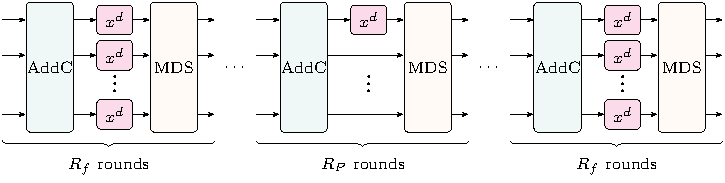
\includegraphics[width=0.9\textwidth]{poseidon_diagram.pdf}
	\caption{Overview of \poseidon and \poseidonnew. (Figure from~\cite{DBLP:phd/hal/Bouvier23})}
	\label{fig:poseidon}
\end{figure}

\paragraph{Attack models used in Section~\ref{Section:Application}.}
We follow the algebraic models from~\cite{DBLP:journals/tosc/GrassiKR25}. The direct Dixon method is applied to the input/output model, while the mixed-degree subspace models are estimated using the Hessenberg bound from Corollary~\ref{cor:three_bounds}(3). This is the reason the \poseidon part of the main text only needs the final complexity plots and timing table.

\newpage
\section{Vision}
\label{appendix:vision}

\vision is a ZK-friendly hash function following the \emph{MARVELlous} design strategy proposed in~\cite{DBLP:journals/tosc/AlyABDS20}. Over $\mathbb{F}_{2^\ell}$, each round alternates inverse maps with affine layers. For $s$ branches, the round functions are
\begin{equation*}
	\begin{aligned}
		\mathcal{F}_{2i}(x) &= \mathsf{M} \cdot \big(B^{-1}(x_0^{-1}), \ldots, B^{-1}(x_{s-1}^{-1})\big) + C_{2i}, \\
		\mathcal{F}_{2i+1}(x) &= \mathsf{M} \cdot \big(B(x_0^{-1}), \ldots, B(x_{s-1}^{-1})\big) + C_{2i+1},
	\end{aligned}
\end{equation*}
where $\mathsf{M}$ is an MDS matrix with rows indexed by $1,\ldots,s$, the $C_j$ are round constants, and $B(x)=b_0+b_1x+b_2x^2+b_3x^4$ is an $\mathbb{F}_2$-affine linearized polynomial.

\begin{figure}[!htbp]
	\centering
	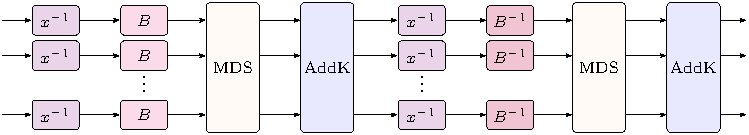
\includegraphics[width=0.9\textwidth]{vision_diagram.pdf}
	\caption{Round function of \vision. (Figure from~\cite{DBLP:phd/hal/Bouvier23})}
	\label{fig:vision}
\end{figure}

\paragraph{MITM model used in Section~\ref{Section:Application}.}
For the CICO problem with $s=2$, we follow the general MITM philosophy of~\cite{DBLP:conf/asiacrypt/LiuMM24} but use Dixon elimination instead of an overdefined-system Gr\"obner-basis attack. The intermediate variables and equations are listed below.

For $r$ rounds, we introduce intermediate variables $(w_{i,1}, w_{i,2})$ and $(z_{i,1}, z_{i,2})$ at round $i$ $(1 \leq i \leq r)$, so that the round-$1$ variables $w_{1,j}$ and $z_{1,1}$ occurring in the input constraint below are covered.
The core equations are:
\begin{equation}
	F^{(1)}_{i,k} := B(w_{i,k}) \cdot \left(\sum_{j=1}^s \mathsf{M}[k][j] \cdot B(z_{i-1,j}) + \epsilon_{i-1,k}\right) - 1,
	\qquad k \in \{1,2\},
\end{equation}
for the first inverse layer, and
\begin{equation}
	F^{(2)}_{i,k} := z_{i,k} \cdot \left(\sum_{j=1}^s \mathsf{M}[k][j] \cdot w_{i,j} + \sigma_{i,k}\right) - 1,
	\qquad k \in \{1,2\},
\end{equation}
for the second inverse layer; $\epsilon_{i,k}$, $\sigma_{i,k}$ and $\beta_{3,1}$ denote the known constants of the corresponding affine layers.

The fixed-input and fixed-output constraints are represented by
\begin{equation}
	f^{(\mathrm{in})} := z_{1,1} \cdot \left(\sum_{j=1}^s \mathsf{M}[1][j] \cdot w_{1,j} + \sigma_{1,1} + \beta_{3,1}\right) - 1,
\end{equation}
and
\begin{equation}
	f^{(\mathrm{out})} := \sum_{j=1}^s \mathsf{M}[1][j] \cdot B(z_{r,j}) + \epsilon_{r,1}.
\end{equation}
Imposing the CICO conditions fixes one input and one output coordinate and removes the corresponding pair of intermediate variables together with the two equations attached to it. What remains is one free input variable together with $2r-1$ pairs of intermediate variables, i.e.\ $4r-1$ variables, and the equations
\[
\underbrace{2r-2}_{\deg=8,\ \text{shape }F^{(1)}}
\;+\;
\underbrace{2r}_{\deg=2,\ \text{shape }F^{(2)}\text{, including }f^{(\mathrm{in})}}
\;+\;
\underbrace{1}_{\deg=4,\ f^{(\mathrm{out})}}
\;=\;4r-1 ,
\]
which is the count split into the forward and backward chains in Table~\ref{tab:vision_equation_distribution}. For $r=2$, for instance, this is $2$ equations of degree $8$, $4$ of degree $2$ and $1$ of degree $4$, matching the instance used in our experiments. This is the shape of the ladder~\eqref{eq:iterative_chain}: $|\mathcal{F}_1|=|\mathcal{X}_0|+1=2$, $|\mathcal{F}_i|=2$ for the remaining rungs, plus the single output constraint.

The equation-degree distribution used in the MITM estimate is summarized in Table~\ref{tab:vision_equation_distribution}.
\begin{table}[!htbp]
	\centering
	\caption{Degree distribution of equations for MITM elimination of \vision. Rows split each round count into the forward and backward chains; the three middle columns give the number of equations of degree $8$, $2$, and $4$ in that chain; the last column reports the total degree of the resultant produced by that chain.}
	\label{tab:vision_equation_distribution}
	\begin{tabular}{cc|c|ccc|c}
		\toprule
		\multirow{2}{*}{$r$} & &\multirow{2}{*}{Equation} & \multicolumn{3}{c|}{\# Equations} & \multirow{2}{*}{Degree} \\
		\cmidrule{4-6}
		& & &$\deg =8$ & $\deg =2$ & $\deg =4$ & \\
		\midrule
		\multirow{2}{*}{even} & &Forward & $r$ & $r$ & $0$ & $2^{4r}$ \\
		& &Backward & $r-2$ & $r$ & $1$ & $2^{4r-4}$ \\
		\midrule
		\multirow{2}{*}{odd} &  &Forward & $r-1$ & $r+1$ & $0$ & $2^{4r-2}$ \\
		& & Backward & $r-1$ & $r-1$ & $1$ & $2^{4r-2}$ \\
		\bottomrule
	\end{tabular}
\end{table}

The MITM elimination proceeds by computing forward resultants up to the middle state and backward resultants from the output side to the same middle state. The two shared middle variables $\mathcal{Z}$ are retained throughout, so the forward chain terminates in one relation in $\mathcal{Z}$ of total degree $D_{\mathrm{fwd}}$ and the backward chain in another of total degree $D_{\mathrm{bwd}}$. The final step is a single resultant within $\mathcal{Z}$: it eliminates one of the two middle variables between these two relations, yielding the univariate eliminant in the remaining middle variable. This is the detailed model underlying Equation~\eqref{eq:mitm_complexity} in the main text.

\paragraph{Rank and extraction cost of a rung.}
Let the incoming relation $R$ have degree at most $D$ in the eliminated
block $\xvec=(x_1,x_2)$, and let the two local equations have block degree
at most $e$.
Expanding the refined cancellation determinant along the column of $R$
gives $\Delta=\sum_{i=1}^3(-1)^{i+1}\widehat C_{i,R}m_i$,
where $m_i$ is the corresponding local $2\times2$ minor.
The three $R$-entries decompose into at most $1,D,D$ products
of a polynomial in $\xvec$ and a polynomial in $\bar{\xvec}$, respectively,
while grouping the local minors by dual monomials gives ranks at most
$e(3e-1)/2$, $\binom{e+1}{2}$ and $e$, respectively. Hence
\begin{equation}\label{eq:rung_rank}
 \operatorname{rank}\mathcal M
 \le r_0:=\frac{e(e+3)}2D+\frac{e(3e-1)}2 .
\end{equation}
The same expansion has $\mathcal{O}(e^4D^3)$ terms and explicitly gives
$\mathcal M=UV$ of inner dimension $r_0$, independently of the
characteristic.
After a rank-preserving specialization, a row basis $U_{I,:}$ gives
$\mathcal M_{I,:}=U_{I,:}V$ with the same row space as $\mathcal M$.
Thin-matrix elimination therefore extracts a maximal-rank submatrix in
$\widetilde{O}(N\bar\rho^{\omega-1})$ operations, where
$\bar\rho=\min\{N,r_0\}$ and $N$ bounds both support dimensions;
use dense elimination if $r_0>N$.
For fixed $e$, the $\widetilde{O}(D^3)$ factor-construction cost is
included in Step~1.

For \vision with $s=2$ the two local equations of a rung have block bidegree $(e,e)$ with $e=1$ for the $\deg=2$ rungs and $e=4$ for the $\deg=8$ rungs, so~\eqref{eq:rung_rank} reads $\rho\le 2D_{\mathrm{in}}+1$ and $\rho\le 14D_{\mathrm{in}}+22$ respectively, against a support dimension $D(\mathcal{F})=\Theta(D_{\mathrm{in}}^{2})$.

\paragraph{Determinant model used in the tables.}
An incoming relation involves only the eliminated block. Each of the two local equations has retained-block degree at most $e$, so a Dixon-matrix entry has retained degree at most $E=2e$. Conditional on the degree bound $D_{\mathrm{out}}$ for the actual determinantal output, put $b=\min\{\bar\rho E,D_{\mathrm{out}}\}$; otherwise use $b=\bar\rho E$. With two retained variables, Kronecker substitution followed by HNF costs
\[
 \widetilde O\!\left(\bar\rho^\omega E(b+1)\right).
\]
This expression gives the Step~4 entries below, including the first rung with $\bar\rho=2,E=2$. The final merge is univariate and uses $\widetilde O(d_{\max}^{\omega}(D_{\mathrm{fwd}}+D_{\mathrm{bwd}}))$. These HNF estimates do not use the point-evaluation interpolation model or its probe cost $L_4$.

\paragraph{Stage-by-stage results.}
Tables~\ref{tab:vision_stages_r4} and~\ref{tab:vision_stages_all} record the cost of every elimination carried out by Method~2, so that the claim of Section~\ref{subsec:method2} that the final merge dominates can be read off directly. For a rung we list the degree $d$ of the local block, the total degrees $D_{\mathrm{in}}$ and $D_{\mathrm{out}}$ of the incoming and outgoing relations, the support dimension $D(\mathcal{F})$ of the associated Dixon matrix, the rank bound $\bar\rho=\min\{D(\mathcal F),r_0\}$ used for Step~3, and the costs of Steps~1, 3 and~4; the cost of the rung is their maximum. Forward rungs are numbered $\mathrm{F}i$ and backward rungs $\mathrm{B}i$ according to their position in the ladder. All entries are $\log_2$ field operations at $\omega=2$. Step~1 uses the $\mathcal{O}(e^4D_{\mathrm{in}}^{3})$ term count above, with fixed-$e$ constants suppressed, which is far below the $\Theta(D(\mathcal{F})^2)$ coefficient positions of a dense Dixon polynomial. For Step~3 we use the rank-sensitive cost model $\widetilde{\mathcal{O}}(D(\mathcal{F})\bar\rho^{\omega-1})$; its estimate remains below Step~4 for the listed parameters. The first rung has no incoming relation $R$ and uses the ordinary two-polynomial bound $N=\bar\rho=2$ instead.

\begin{table}[ht]
	\centering
	\small
	\caption{Every Dixon elimination performed by Method~2 on \vision with $r=4$ ($s=2$), in $\log_2$ field operations, $\omega=2$. The meet-in-the-middle cut is after rung~$4$.}
	\label{tab:vision_stages_r4}
	\setlength{\tabcolsep}{4pt}
	\renewcommand{\arraystretch}{1.1}
	\begin{tabular}{lccccccccc}
		\toprule
		Stage & $d$ & $\log_2 D_{\mathrm{in}}$ & $\log_2 D_{\mathrm{out}}$ & $\log_2 D(\mathcal{F})$ & $\log_2\bar\rho$ & Step~1 & Step~3 & Step~4 & Cost \\
		\midrule
		F1    & $2$ & $0$  & $2$  & $1.0$  & $1.0$  & $3.0$  & $2.0$  & $5.3$  & $5.3$ \\
		F2    & $8$ & $2$  & $8$  & $4.5$  & $4.5$  & $6.0$  & $8.9$  & $19.4$ & $19.4$ \\
		F3    & $2$ & $8$  & $10$ & $15.0$ & $9.0$  & $24.0$ & $24.0$ & $29.0$ & $29.0$ \\
		F4    & $8$ & $10$ & $16$ & $19.0$ & $13.8$ & $30.0$ & $32.8$ & $46.6$ & $46.6$ \\
		\midrule
		B7    & $2$ & $2$  & $4$  & $3.3$  & $3.2$  & $6.0$  & $6.5$  & $11.4$ & $11.4$ \\
		B6    & $8$ & $4$  & $10$ & $7.5$  & $7.5$  & $12.0$ & $15.0$ & $28.0$ & $28.0$ \\
		B5    & $2$ & $10$ & $12$ & $19.0$ & $11.0$ & $30.0$ & $30.0$ & $35.0$ & $35.0$ \\
		\midrule
		Merge & --- & $16$ & ---  & $16.0$ & $16.0$ & $48.0$ & $32.0$ & $48.1$ & $\mathbf{48.1}$ \\
		\bottomrule
	\end{tabular}
\end{table}

\begin{table}[ht]
	\centering
	\small
	\caption{Maximal forward and backward stage cost against the final merge, for \vision with $s=2$ and $2\le r\le 10$, in $\log_2$ field operations, $\omega=2$. The last column is the complexity reported for Method~2.}
	\label{tab:vision_stages_all}
	\setlength{\tabcolsep}{4pt}
	\renewcommand{\arraystretch}{1.1}
	\begin{tabular}{@{}ccccccc@{}}
		\toprule
		$r$ & $\log_2 D_{\mathrm{fwd}}$ & $\log_2 D_{\mathrm{bwd}}$ & Max.\ forward & Max.\ backward & Merge & Max.\ over stages \\
		\midrule
		$2$  & $8$  & $4$  & $19.4$  & $11.4$  & $24.1$  & $24.1$ \\
		$3$  & $10$ & $10$ & $29.0$  & $28.0$  & $31.0$  & $31.0$ \\
		$4$  & $16$ & $12$ & $46.6$  & $35.0$  & $48.1$  & $48.1$ \\
		$5$  & $18$ & $18$ & $53.0$  & $52.6$  & $55.0$  & $55.0$ \\
		$6$  & $24$ & $20$ & $70.6$  & $59.0$  & $72.1$  & $72.1$ \\
		$7$  & $26$ & $26$ & $77.0$  & $76.6$  & $79.0$  & $79.0$ \\
		$8$  & $32$ & $28$ & $94.6$  & $83.0$  & $96.1$  & $96.1$ \\
		$9$  & $34$ & $34$ & $101.0$ & $100.6$ & $103.0$ & $103.0$ \\
		$10$ & $40$ & $36$ & $118.6$ & $107.0$ & $120.1$ & $120.1$ \\
		\bottomrule
	\end{tabular}
\end{table}

The candidate roots of the final univariate eliminant are substituted back into the original system, which removes the spurious ones at negligible additional cost.

\newpage
\section{\texorpdfstring{\xhash}{XHash12}}
\label{appendix:xhash}

\xhash is a STARK-friendly sponge hash function proposed by Ashur et al.~\cite{DBLP:journals/iacr/AshurKM23}. The permutation over $\mathbb{F}_p^{12}$ is
\[
\mathcal{F}(x) =  M\circ \mathcal{B}_2 \circ \mathcal{I}_2\circ \mathcal{P}_2 \circ  \mathcal{B}_1 \circ \mathcal{I}_1\circ \mathcal{P}_1 \circ \mathcal{B}_0 \circ  \mathcal{I}_0\circ \mathcal{P}_0(x),
\]
where $p = 2^{64}-2^{32}+1$. The nonlinear layers combine power maps over $\mathbb{F}_p$ and over $\mathbb{F}_{p^3}$.

\begin{figure}[!htbp]
	\centering
	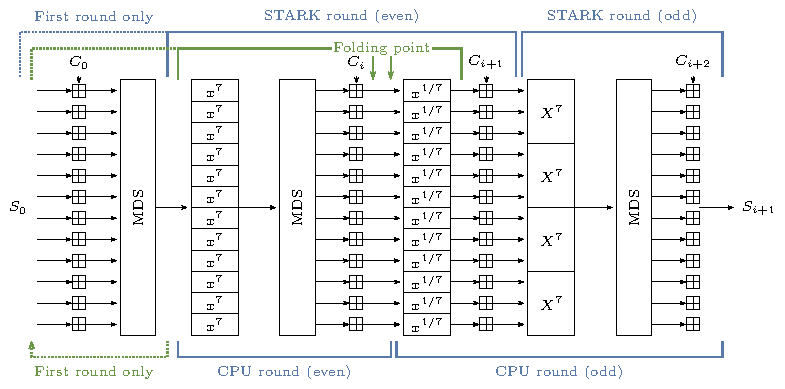
\includegraphics[width=0.95\textwidth]{xhash12_diagram.pdf}
	\caption{Round function of \xhash~\cite{DBLP:journals/iacr/AshurKM23}}
	\label{fig:xhash12}
\end{figure}

\paragraph{Hybrid model used in Section~\ref{Section:Application}.}
For an $s$-step instance, let $n=12s$ and write the system in triangular form
\[
\mathcal{P}_k = \left\{
\begin{array}{l}
	Z_1^\alpha - f_1(\mathcal{X}) = 0 \\
	\vdots \\
	Z_n^\alpha - f_n(\mathcal{X}, Z_1, \ldots, Z_{n-1}) = 0 \\
	h_1(\mathcal{X}, Z_1, \ldots, Z_n) = 0 \\
	\vdots \\
	h_k(\mathcal{X}, Z_1, \ldots, Z_n) = 0
\end{array}
\right.
\]
with $\alpha=7$ for the standard \xhash instance. The complexity curves use $\bar D=\alpha$ for the output constraints and the degree bounds $D_i=\alpha^{n-i}\bar D$ before each successive elimination. For CICO-1, we instantiate~\eqref{eq:two_poly_complexity_main} with $d_{\mathcal I}=\alpha^n$. For $k\ge2$, we evaluate the sum in~\eqref{eq:successive_elim_cost} and bound the final relation degrees by $\alpha^n\bar D$. In both the direct and final hybrid Dixon computations, construction uses the cheaper of Kronecker$+$HNF and cached expansion, followed by rank extraction and univariate HNF; the reported estimate is the maximum over these stages.

\subsection{Multivariate Reduction and Elimination Costs}\label{appendix:hybrid_cost_proof}
Fix $\alpha\ge2$ and the number $k$ of retained variables $\mathcal X=(X_1,\ldots,X_k)$. Let $\mathcal P_i=\{z_j^\alpha-f_j:1\le j\le i\}$ be a reduced triangular system. Give each $X_j$ weight $1$ and choose nonnegative weights $w_i$ recursively so that $d_w(f_i)\le\alpha w_i$. Thus reduction cannot increase weighted degree, and the total degree in $\mathcal X$ is bounded by weighted degree. Assume $\deg_{z_i}h_j\le2\alpha-2$ and $\bar D=\max_j d_w(h_j)\ge1$. The estimates below have constants depending on the fixed $\alpha,k$.

\emph{Reduction.}
For a polynomial of weighted degree at most $D$ with $\deg_{z_j}\le2\alpha-2$, every intermediate retained-variable degree in \texttt{Reduce} is at most $D$. Products of reduced coefficients can be encoded in a box with at most $(D+1)^k(2\alpha-1)^{i-1}$ positions. Since $(D+1)^k=O_k(B_k(D))$, fast multiplication costs $\widetilde O_k(B_k(D)(2\alpha-1)^{i-1})$. The recurrence of~\cite[Proposition~3 and Lemma~1]{DBLP:conf/crypto/BariantBBHOR25} therefore becomes
\[
 C_i(D)\le(2\alpha-1)C_{i-1}(D)
 +\widetilde O_{\alpha,k}\!\left(B_k(D)(2\alpha-1)^{i-1}\right),\qquad C_0(D)=0.
\]
Unfolding it gives $C_i(D)=\widetilde O_{\alpha,k}(B_k(D)(2\alpha-1)^i)$; the factor $i$ is logarithmic in the coefficient-box size. This proves~\eqref{eq:reduction_cost}. It also bounds multiplication followed by reduction, with $D$ the sum of the two input weighted-degree bounds.

\emph{One resultant.}
Let $h_i$ be reduced modulo $\mathcal P_i$ with $d_w(h_i)\le D_i$. Over $A=\mathbb K[\mathcal X,z_1,\ldots,z_{i-1}]/\langle\mathcal P_{i-1}\rangle$, multiplication by $h_i$ in the free rank-$\alpha$ algebra $A[z_i]/(z_i^\alpha-f_i)$ defines an $\alpha\times\alpha$ matrix. Its determinant equals $\operatorname{Res}_{z_i}(z_i^\alpha-f_i,h_i)$, and hence the resultant used in the text up to a nonzero sign. In the basis $1,z_i,\ldots,z_i^{\alpha-1}$, the entry in row $r$, column $c$ has weight at most $D_i+(c-r)w_i$. Each determinant term consequently has weight at most $\alpha D_i$. If $h_i$ depends on $z_i$, then $w_i\le D_i$, so a division-free determinant computation of this fixed-size matrix involves only weighted degrees $O_\alpha(D_i)$ and $O_\alpha(1)$ multiplications and reductions. If $h_i$ is independent of $z_i$, the determinant is simply $h_i^\alpha$. The reduction bound above gives, in either case,
\[
 \widetilde O_{\alpha,k}\!\left(B_k(D_i)(2\alpha-1)^{i+2}\right).
\]
This supplies the fixed-$\alpha,k$ multivariate counterpart of~\cite[Lemma~2]{DBLP:conf/crypto/BariantBBHOR25}, without requiring roots of unity in the base field.

\emph{Successive stages.}
The weight bound gives $d_w(h_{i-1})\le\alpha d_w(h_i)$, so $D_i=\alpha^{n-i}\bar D$ is valid, as in~\cite[Lemma~3]{DBLP:conf/crypto/BariantBBHOR25}. Summing the one-stage cost over $i$ and the $k$ constraints proves~\eqref{eq:successive_elim_cost}; the final relations have total degree at most $\alpha^n\bar D$. For $k=1$, successive terms in decreasing $i$ have ratio $\alpha/(2\alpha-1)<1$, so the first stage dominates, recovering~\cite[Proposition~7]{DBLP:conf/crypto/BariantBBHOR25}. For fixed $k\ge2$, $B_k(D_i)=\Theta_k(D_i^k)$ and $\alpha^k/(2\alpha-1)>1$, so the last stage dominates. The reduction cost is bounded by the $i=n$ term of the elimination sum.

For CICO-1, the reduction method of~\cite{DBLP:conf/crypto/BariantBBHOR25} can be applied directly. For larger $k$, the hybrid strategy first derives reduced relations $R_1(\mathcal{X}),\ldots,R_k(\mathcal{X})$ from the triangular ideal and then performs a final Dixon elimination on these relations. The hybrid strategy is effective for very small $k$, while direct Dixon elimination gives the better estimate for CICO-4. The reference point for both is the direct Gr\"obner-basis attack of the designers~\cite{DBLP:journals/iacr/AshurKM23}; the same triangular model, with the power maps of $\mathcal{B}_i$ replaced accordingly, applies verbatim to \texttt{XHash8}.
